% !TeX spellcheck = en_GB

\documentclass[proc]{edpsmath}
\usepackage[utf8]{inputenc}
\usepackage[T1]{fontenc}

\usepackage{amsmath,amssymb,amsthm}
\usepackage{graphicx}
\usepackage{hyperref}
\usepackage{physics}

\newcommand{\bR}{\mathbb{R}}
\newcommand{\bb}{\mathbf{b}}
\newcommand{\bA}{\mathbf{A}}
\newcommand{\vp}{v_\parallel}
\newcommand{\bx}{\mathbf{x}}
\newcommand{\bv}{\mathbf{v}}
\newcommand{\bu}{\mathbf{u}}
\newcommand{\bB}{\mathbf{B}}
\newcommand{\Dt}{\Delta t \;}

\newcommand{\dbx}{\dot{\mathbf{x}}}
\newcommand{\diff}[2]{\frac{\text{d} #1}{\text{d} #2}}
\newcommand{\pa}[2]{\frac{\partial #1}{\partial #2}}
\newcommand{\ap}{a_\parallel}
\newcommand{\mean}[1]{\langle #1 \rangle}
\newcommand{\Bap}{B_\parallel^\ast}
\newcommand{\bracket}[2]{\left\{ #1, #2 \right\}}
\newcommand{\gcbracket}[2]{\left\{ #1, #2 \right\}_{\text{g.c.}}}
\newcommand{\dt}{\frac{\text{d}}{\text{d} t}}

\renewcommand{\d}{\;\text{d}}


\begin{document}

\title{SILAS - Semi-Lagrangian scheme with Arakawa splitting}
\thanks{CEMRACS}\thanks{Max-Planck}% At most 5 thanks
%
\author{Dominik Bell}\address{Max-Planck-Institut für Plasmaphysik, Garching, Germany; \email{dominik.bell@ipp.mpg.de\ \&\ frederik.schnack@ipp.mpg.de\ \&\ martin.campos-pinto@ipp.mpg.de\ \&\ sonnen@ipp.mpg.de}}\secondaddress{Technische Universität München, Zentrum Mathematik, Garching, Germany}
\author{Martin Campos Pinto}\sameaddress{1}
\author{Davor Kumozec}\address{Faculty of Sciences, University of Novi Sad, Serbia; \email{davor.kumozec@dmi.uns.ac.rs}}
\author{Frederik Schnack}\sameaddress{1}
\author{Eric Sonnendrücker}\sameaddress{1,2}

\begin{abstract}
In practice, there are various ways to solve gyro-kinetic equations. Here, we will combine the Semi-Lagrangian (SL) method and the Arakawa scheme. Both schemes are successfully implemented in practice when applied individually, but our goal is to decompose the problem into fast (parallel) dynamic and slow (perpendicular) dynamic and to combine these two schemes. The SL scheme will be used to solve the fast subsystem and the Arakawa scheme for the slow one. In our reference code \cite{pygyro_code} the entire model is solved using SL; we will replace the part related to the slow subsystem with an Arakawa scheme. The main reason for combining these two schemes is to get a solution that preserves some of the basic measures in the system we have. In Section II we will describe properties of both schemes and splitting between advection equations. In Part III numerical experiments will be presented, first for the Arakawa scheme as a verification of theoretical properties, and after that for the PyGyro model.
\end{abstract}

\begin{resume}
	En pratique, il existe plusieurs façons de résoudre les équations gyro-cinétiques. Ici, nous allons combiner la méthode Semi-Lagrangienne (SL) et le schéma d'Arakawa. Les deux schémas sont mis en œuvre avec succès dans la pratique lorsqu'ils sont appliqués individuellement, mais notre objectif est de décomposer le problème en dynamique rapide (parallèle) et dynamique lente (perpendiculaire) et de combiner ces deux schémas. Le schéma SL sera utilisé pour résoudre le sous-système rapide et le schéma d'Arakawa pour le lent. Dans notre code de référence \cite{pygyro_code}, le modèle entier est résolu en utilisant la méthode SL; nous remplacerons la partie relative au sous-système lent par un schéma d'Arakawa. La raison principale de la combinaison de ces deux schémas est d'obtenir une solution qui préserve des mesures de base du système que nous avons. Dans la partie II, nous décrirons les propriétés des deux schémas et le fractionnement entre les équations d'advection. Dans la partie III, des expériences numériques seront présentées, d'abord pour le schéma d'Arakawa comme vérification des propriétés théoriques, et ensuite pour le modèle PyGyro.
\end{resume}

\maketitle

\newpage

%\tableofcontents %TODO: can also be removed later

% !TeX spellcheck = en_GB

\section{Introduction}
\label{sec:introduction}
\subsection{The Gyro-kinetic Model}

In a Tokamak, particles have complicated dynamics in real space which consists of a slow motion along the magnetic field lines superimposed with a fast motion circling around the magnetic field lines. This second, fast motion is called gyration and can be averaged out to reduce the dimension of phase space in order to make the models more computationally feasible while keeping most of the important physics. The resulting theory is called a gyro-kinetic model which will be discussed in the following.\\
The model is defined by the Lie-transformed, low-frequency particle Lagrangian $L$ (see \cite{Bottino_Sonnendrucker_2015}):
\begin{equation}\label{Lagrangian}
	L = \left(e\bA + m \vp \bb \right)\cdot\dbx + \frac{m\sqrt{4\pi}}{e \mu_0^{\frac{3}{2}}} \mu \dot{\theta} - H(\bx, \vp)
\end{equation}
with the variables $\bx \in \Omega \subseteq \bR^3$, the position of the gyro-centre, $\vp \in \bR^3$, the velocity parallel to the magnetic field lines, and $\mu$, the modified magnetic moment. $\bA$ will denote the background vector potential. The Hamiltonian $H$ will be discussed below.\\
From the equation of motion for $\theta$ it can be seen immediately that $\mu$ is a constant of the system:
\begin{equation}
	\diff{}{t} \mu = 0
\end{equation}
and phase space is thus 4-dimensional.\\
A kinetic equation for this model is the gyro-kinetic equation for the gyro-centre distribution function $f=f(t,\bx, \vp, \mu)$:
\begin{equation}\label{drift-kinetic model}
	\pa{f}{t} + \bu \cdot \nabla f + \ap \pa{f}{\vp} = 0.
\end{equation}
This function describes the positions of a collection of identical particles of charge $q\neq0$ and mass $m>0$, immersed in a static magnetic field $B(x)$.
The phase-space gyro-centre Hamiltonian $H(\bx, \vp)$ reads
\begin{equation}
	H(t, \bx, \vp, \mu) = \frac{1}{2} m \vp^2 + \mu B(\bx) + q \mean{\phi}_\alpha (t,\bx)
\end{equation}
where the bracket denotes averaging over the gyro-angle $\alpha$: $\mean{\;\cdot\;}_\alpha \equiv \int \cdot\d \alpha / (2\pi)$.\\
Defining
\begin{subequations}
	\begin{align}
		\bA^\ast & \equiv \bA + \frac{m}{e} \vp \bb \\
		\bB^\ast & = \nabla \times \bA^\ast \\
		\Bap & = \bb \cdot \bB = B + \frac{m \vp}{q B} \bb \cdot \left( \nabla \times \bB \right)
	\end{align}
\end{subequations}
one can easily derive the equations of motion from \eqref{Lagrangian}, which then read
\begin{subequations}
	\begin{align}
		\bu = \dbx & = \frac{1}{\Bap} \left( \frac{1}{m} \pa{H}{\vp} \bB^\ast + \frac{1}{q} \bb \times \left(\nabla H\right) \right) \label{eom for bu} \\
		\ap = \dot{\vp} & = \frac{1}{\Bap} \left( -\frac{1}{m} \bB^\ast \cdot \left( \nabla H \right) \right). \label{eom for ap}
	\end{align}
\end{subequations}
As noted in \cite{Latu_2017}, the phase space is divergence-free
\begin{equation}
	\nabla \cdot \bu + \pa{\ap}{\vp} = 0
\end{equation}
i.e. we can rewrite \eqref{drift-kinetic model} in conservative form
\begin{equation}\label{conservation1}
	\pa{}{t}\left(\Bap f\right) + \nabla\cdot\left( \Bap \bu f \right) + \pa{}{\vp} \left( \Bap \ap f \right) = 0.
\end{equation}
Splitting between fast and slow steps yields:
\begin{subequations}
	\begin{align}
		(\text{fast}) = & \left\{ \begin{aligned}
			\bu_f & = \frac{1}{\Bap} \frac{1}{m} \pa{H}{\vp} \bB \\
			a_{\parallel, f} & = -\frac{1}{\Bap} \frac{1}{m} \bB \cdot \left( \nabla H \right)
		\end{aligned} \right. \label{split step fast}\\
		(\text{slow}) = &  \left\{ \begin{aligned}
			\bu_s & = \frac{1}{\Bap} \frac{1}{q} \left( \pa{H}{\vp} \vp \nabla \times \bb + \bb \times \left(\nabla H\right) \right) \\
			a_{\parallel, s} & = - \frac{a}{\Bap} \frac{1}{q} \vp \left( \nabla \times \bb \right) \cdot \left( \nabla H \right)
		\end{aligned} \right. \label{split step slow}
	\end{align}
\end{subequations}
Both fast and slow steps are divergence-free and derived from a Poisson bracket.\\
The guiding-centre Poisson bracket reads:
\begin{subequations}
	\begin{align}
		\gcbracket{F}{G} & = \frac{\bB^\ast}{m \Bap} \cdot \left( \left(\nabla F\right) \pa{G}{\vp} - \left(\nabla G\right) \pa{F}{\vp} \right) \label{gc Pb part 1} \\
		& \qquad + \frac{\vp}{q \Bap} \left( \nabla \times \bb \right) \cdot \left( \left(\nabla F\right) \pa{G}{\vp} - \left(\nabla G\right) \pa{G}{\vp} \right) \label{gc Pb part 2} \\
		& \qquad - \frac{1}{q \Bap} \bb \cdot \left[\left(\nabla F\right) \times \left(\nabla G\right)\right]. \label{gc Pb part 3}
	\end{align}
\end{subequations}
For a constant background magnetic field $\bB$, the model is simplified and the fast and slow steps become 
\begin{subequations}
	\begin{align}
		(\text{fast}) = & \left\{ \begin{aligned}
			\bu_f & = {\vp} \bb \\
			a_{\parallel, f} & = -\frac{q}{m} \bb \cdot \nabla \phi
		\end{aligned} \right. \label{split step fast const B}\\
		(\text{slow}) = &  \left\{ \begin{aligned}
			\bu_s & = \frac{\nabla \phi\times \bb}{\bB}  \\
			a_{\parallel, s} & = 0
		\end{aligned} \right. \label{split step slow const B}
	\end{align}
\end{subequations}
We refer to \cite{Latu_2017} for some background on the model. The aim is to look for $f = f(t, r, \theta, z, v_\parallel)$ satisfying
\begin{equation}
\partial_t f + \{\phi, f\} + v_\parallel \nabla_\parallel - \nabla_\parallel \phi \partial_{v_\parallel}f = 0, \label{eq:GK_model}
\end{equation}
where $\nabla_\parallel = \bb \cdot \nabla$ and the bracket is in polar coordinates
\begin{equation}
\{\phi, f \} = \frac{1}{rB_0}\partial_r \phi\partial_\theta f -\frac{1}{rB_0}\partial_\theta \phi\partial_r f. \label{eq:bracket_in_polar}
\end{equation}
Since the plasma is quasi-neutral, what means that locally there may be charged regions but it is neutral overall, we can express self-consistent potential $\phi = \phi(t, r, \phi, z)$ as a solution to the following Poisson type, quasi-neutrality (QN) equation (for more details see \cite{emily})
\begin{equation}
- \left[\partial_r^2 \phi + \left( \frac{1}{r} + \frac{\partial_r n_0}{n_0}\right)\partial_r \phi + \frac{1}{r^2} \partial_\theta^2 \phi \right] + \frac{1}{T_e} \phi = \int_{-\infty}^{\infty} (f - f_\text{eq}) \ \dd v_\parallel. \label{eq:qn}
\end{equation}
This equation will be treated using finite element method (FEM) on a B-spline basis. The independence of the equation from the $z$ direction and the periodicity of the solution in $\theta$ direction will be used to parallelize the code.

\subsection{Boundary Conditions and Conservation Laws}

Boundary conditions on $f$ are
\begin{itemize}
    \item Periodicity along $\theta$ and $z$.
    \item Boundary conditions along $v_\parallel$ are cubic spline approximation of the distribution function %TODO
    \item In $r$ direction, either Dirichlet boundary conditions (for the second-order scheme only) or extrapolation to an outside equilibrium function
\end{itemize}

For the boundary conditions on $\phi$ we take
\begin{itemize}
    \item Periodic along $\theta$.
    \item Boundary Conditions along $z$ %TODO...QN equation does not depend on the $z$ so I think we dont need this here or just to say that it is periodic again as in function f
    \item In $r$-direction, $\phi$ is decomposed into Fourier modes. At $r_\text{min}$, we take homogeneous Neumann boundary conditions for the zeroth mode and homogeneous boundary conditions for the others. At $r_\text{max}$, we just take homogeneous Dirichlet boundary conditions.
\end{itemize}

\textbf{Conserved Quantities}\\
Firstly, we have a transport equation in conservative form \eqref{conservation1}. Secondly, \eqref{drift-kinetic model} conserves arbitrary functions of $f$  along nonlinear characteristics,
\begin{equation}
\dt C(f) + \bracket{C(f)}{H} =0,
\end{equation}
and the Casimir invariant $\int C( f ) d^5R$ is also conserved. Therefore, in addition to the particle number or the $L^1$-norm $\int f d^5R$, the system has an infinite number of conserved quantities such as the $L^2$-norm $\int f^2 d^5R$, and the kinetic entropy $S=\int f \ln(f) d^5R$.\\
Thirdly, the gyrokinetic equations conserve the total energy $H = E_k + E_f$:
\begin{subequations}
	\begin{align}
		E_k &= \frac{1}{2} m \vp^2 + \mu B(\bx),\\
		E_f &= q \mean{\phi}_\alpha (t,\bx).
	\end{align}
\end{subequations}
where $E_k$ is the kinetic energy and $E_f$ is the field energy. For more details on this, we refer the reader to \cite{idomura2008conservative}.\\

In the next chapter we will explain the numerical scheme used to obtain the approximate solution of the GK model. Our goal is combine the Semi-Lagrangian (SL) and Arakawa scheme (AK). SL scheme will be used to solve fast subsystem and AK for slow. The main reason for combining these two schemes is to get a solution that preserves some of the basic measures in the system we have.

% !TeX spellcheck = en_GB

\section{Operator Splitting and Discretization}
\label{sec:splitting_discretization}

It is a common tool to split a PDE in several sub-steps in order to do the numerical integration. This simplifies the equation tremendously at the cost of introducing some numerical error. Multiple sub-flows can be recombined to yield an approximation to a time-step of the full PDE; most commonly used methods for this are the \textbf{Strang splitting} which is of first order, and \textbf{Lie splitting} which is a second order method (for more details see \cite{emily}). In the code \cite{pygyro_code} Lie splitting is used for a predictor step and then Strang splitting to compute the full time-step from the predicted distribution function.


We can split our equation 
\begin{equation}
 \partial_t f + \{\phi, f \} + v_\parallel \nabla_\parallel f - \nabla_\parallel \phi\,\, \partial_{v_\parallel} f = 0
\end{equation}
for the distribution function $f$ into three advection equations:
\begin{subequations}
	\begin{align}
		\partial_t f + v_\parallel \nabla_\parallel f & = 0 && \text{Advection on flux surface} & \\
		\partial_t f + \nabla_\parallel \phi\,\, \partial_{v_{\parallel}} f & = 0 && \text{V-parallel advection} & \\
		\partial_t f + \{\phi, f\} & = 0 && \text{Advection on poloidal plane} \label{eq:adv_poloidal} &
	\end{align}
\end{subequations}
where $\{\phi,f\}$ is a Poisson bracket, defined as follows:
\begin{equation}
 \{\phi,f\}=-\frac{\partial_\theta\phi}{rB_0}\partial_r f + \frac{\partial_r\phi}{rB_0}\partial_\theta f.
\end{equation}
In our work, we will use two different approaches to solving these equations. For the first two we will use the semi-Lagrangian scheme and for the third equation we will use the Arakawa scheme. The reason for different approaches in solving these three equations is that most of the physical properties like preservation of the mass, $L_2$ norm and total energy, are happening in the \eqref{eq:adv_poloidal}. For the semi-Lagrangian scheme we know that it is unconditionally stable, but it does not preserve these quantities, so for the equation \eqref{eq:adv_poloidal} we implemented the Arakawa scheme which is known to hold these properties.







\subsection{Semi-Lagrangian Scheme for the Fast Time Subsystem}
%TODO: What are the conservation properties of the SL scheme
The fast time subsystem will be solved using semi-Lagrangian scheme. As reference we will use \cite{campospinto} and \cite{emily}.
The code for this part can be found at \cite{pygyro_code}. We will use general notations in the beginning and then move on to the specific problem we have in our model. This scheme is frequently used in solving advection problems of the form:
\begin{equation}
    \partial_t f(t,\mathbf{x})+v(t,\mathbf{x})\cdot \nabla f(t,\mathbf{x})=0, \qquad t\in[0,T], \quad \mathbf{x}\in\mathbb{R}^d
\end{equation}
where $v$ is a velocity field $\mathbb{R}^d\longrightarrow\mathbb{R}^d$, $T$ is a final time, and initial conditions are given by $f_0(\mathbf{x})=f(0,\mathbf{x})$. For simplicity, we will assume that $v$ is given and smooth enough so we can use the method of characteristics. Thus we can obtain the trajectories $X(t)=X(t;s,x)$ as a solutions to ODE
\begin{equation}
    X'(t)=v(t,X(t)), \qquad X(s)=x, \qquad t\in[0,T].
\end{equation}
It can be shown that the flow $F_{s,t}:x\longrightarrow X(t)$ is invertible and satisfies $(F_{s,t})^{-1}=F_{t,s}$. We know that the analytical solution to our equation is given by
\begin{equation}
    f(t,\mathbf{x})=f_0((F_{0,t})^{-1}(\bx)),\qquad \text{for } t\in[0,T], \quad \mathbf{x}\in\mathbb{R}^d.
\end{equation}
Now we are using backward tracking of the characteristic
\begin{equation}
    B^{n,n+1}=(F_{t_n,t_{n+1}})^{-1}
\end{equation}
between two time steps $t_n=n\Delta t$ and $t_{n+1}$. For the last step we have to approximate the function $f$ at the grid points $f^n=f(t_n)$. For this purpose, we will use splines.

The flux surface advection operator defined by the equation
\begin{equation}
 \partial_t f + v_\parallel \nabla_\parallel f = 0
\end{equation}
and is a two-dimensional semi-Lagrangian operator. Here we can determine the exact trajectory because the velocity in the equation is constant and is not related to the surface of the flux.

In order to determine the value of the distribution function in the discretization grid for characteristics that go outside our domain, we use a combination of a one-dimensional cubic spline and a Lagrangian interpolation polynomial of fifth order in $\theta$ and $z$ directions, respectively. In this way, we get an approximation of the value of the function in the final position.

The v$_\parallel$ surface advection operator defined by equation
\begin{equation}
    \partial_t f + \nabla_\parallel \phi\,\, \partial_{v_{\parallel}} f = 0
\end{equation}
and is a one-dimensional semi-Lagrangian operator. Here we use a cubic spline to determine the value of the particle distribution function for characteristics that go outside the domain. The parallel gradient of $\phi$ depends only on the spatial coordinates and is therefore constant along the surface $v_\parallel$. As a result, the trajectory used by the semi-Lagrangian method can be accurately defined. The parallel gradient of $\phi$ is computed using a (field-aligned) finite difference method of order 6 in the $z$ direction. This was calculated as described by Latu et al. \cite{Latu_2017}.







\subsection{Arakawa Scheme for the Slow Time Subsystem}

For the Arakawa scheme, we mainly reference the article \cite{Arakawa_1966}. Here we are interested in solving the advection on poloidal plane:
\begin{equation}
 \partial_t f + \{\phi, f\} = 0
\end{equation}
where $\{\phi,f\}$ is a Poisson bracket, defined as follows:
\begin{equation}\label{eq:poisson_bracket}
	 \{\phi,f\} = - \frac{1}{rB_0} \left(\partial_\theta\phi\right) \left(\partial_r f\right) + \frac{1}{rB_0} \left(\partial_r\phi\right) \left(\partial_\theta f\right) \, .
\end{equation}
The Arakawa scheme provably preserves the following quantities:
	\begin{align}\label{conservation-properties}
		\text{mass} : && \dt \int f(t) \d x \text{d} y & = 0 & \Leftrightarrow && \int\bracket{\phi}{f} \d x \text{d} y & = 0\\
		L^2\text{-norm :} && \dt \int f^2(t) \d x \text{d} y & = 0 & \Leftrightarrow && \int f \, \bracket{\phi}{f} \d x \text{d} y & = 0\\
		\text{total energy :} && \dt \int \phi \, f(t) \d x \text{d} y & = 0 & \Leftrightarrow && \int \phi \bracket{\phi}{f} \d x \text{d} y & = 0
	\end{align}
First we will focus on discretization of Poisson bracket in Cartesian coordinates. The scheme in polar coordinates will be discussed below.







\subsubsection{Construction of a Discrete Bracket using the Arakawa Method}

The first step in constructing the 4th order Arakawa scheme is to explain second order discretization using nine point stencil. We have approximation of $J(f,g)$ at $(i,j)$ of the following form
\begin{equation}
J(f,g)=\frac{1}{3}(J^{++}+J^{+\times}+J^{\times+})+\mathcal{O}(d^2)
\end{equation}
where
\begin{equation}
    J^{++}_{ij}=\frac{1}{4d^2}[(f_{i+1,j}-f_{i-1,j})(g_{i,j+1}-g_{i,j-1})-(f_{i,j+1}-f_{i,j-1})(g_{i+1,j}-g_{i-1,j})],
\end{equation}
\begin{equation}
    \begin{aligned}
    	J^{+\times}_{ij} & = \frac{1}{4d^2} \left[ f_{i+1,j} (g_{i+1,j+1} - g_{i+1,j-1}) - f_{i-1,j} (g_{i-1,j+1} - g_{i-1,j-1}) \right. \\
    	& \hspace{11mm} \left. - f_{i,j+1} (g_{i+1,j+1} - g_{i-1,j+1}) + f_{i,j-1}(g_{i+1,j-1} - g_{i-1,j-1}) \right]
    \end{aligned}
\end{equation}
and
\begin{equation}
    \begin{aligned}
    	J^{\times+}_{ij} & = \frac{1}{4d^2} \left[ f_{i+1,j+1} (g_{i,j+1} - g_{i+1,j}) - f_{i-1,j-1} (g_{i-1,j} - g_{i,j-1}) \right. \\
    	& \hspace{11mm} \left. - f_{i-1,j+1} (g_{i,j+1} - g_{i-1,j}) + f_{i+1,j-1} (g_{i+1,j} - g_{i,j-1}) \right]
    \end{aligned}
\end{equation}
We denote the linear combination $J_1=\frac{1}{3}(J^{++}+J^{+\times}+J^{\times+})$, which is a second order approximation conserving the square of vorticity and the energy.

In order to extend the discretization to 4th order we introduce $J_2=\frac{1}{3}(J^{\times \times} + J^{\times+} + J^{+\times})$ where we use the same nine point stencil with the additional
four points $(i+2,j)$, $(i-2,j)$, $(i,j+2)$  and $(i,j-2)$ for $J_2$, where
\begin{equation}
	J^{\times\times}_{ij} = \frac{1}{8d^2} \left[(f_{i+1,j+1} - f_{i-1,j-1}) (g_{i-1,j+1} - g_{i+1,j-1}) - (f_{i-1,j+1} - f_{i+1,j-1}) (g_{i+1,j+1} - g_{i-1,j-1}) \right] \, ,
\end{equation}
\begin{equation}
	\begin{aligned}
		J^{\times+}_{ij} & = \frac{1}{8d^2} \left[ f_{i+1,j+1} (g_{i,j+2} - g_{i+2,j}) - f_{i-1,j-1} (g_{i-2,j} - g_{i,j-2}) \right. \\
		& \hspace{11mm} \left. - f_{i-1,j+1} (g_{i,j+2} - g_{i-2,j}) + f_{i+1,j-1} (g_{i+2,j} - g_{i,j-2})\right] \, ,
	\end{aligned}
\end{equation}
and
\begin{equation}
	\begin{aligned}
		J^{+\times}_{ij} & = \frac{1}{8d^2} \left[f_{i+2,j} (g_{i+1,j+1} - g_{i+1,j-1}) - f_{i-2,j} (g_{i-1,j+1} - g_{i-1,j-1}) \right. \\
		& \hspace{11mm} \left. - f_{i,j+2} (g_{i+1,j+1} - g_{i-1,j+1}) + f_{i,j-2} (g_{i+1,j-1} - g_{i-1,j-1})\right] \, .
	\end{aligned}
\end{equation}
By Taylor extension, we can see that $2J_1-J_2$ is a fourth order approximation of the Jacobian $J$; that is,
$2J_1-J_2=J+O(d^4)$.
Now we have the second-order nine-point scheme and the fourth-order thirteen-point scheme. For the proof of the stencil order, we refer to appendix \ref{sec:ara_order}.







\subsubsection{Boundary Conditions}

Let show first what is happening if $g$ is constant at boundary. By
\begin{equation}
    J_{ij}(f,g)=\sum^*_{i',j'}[a_{i,j;i+i',j+j'}(f_{i+i',j+j'}+f_{i,j})-a_{i-i',j-j';i,j}(f_{i,j}+f_{i-i',j-j'})].
\end{equation}
and assume $g$ is constant at the boundary $j=0$ (and outside of the domain), the discrete Jacobian is treated as
\begin{equation}
\begin{aligned}
\frac{1}{2}J_{i0} (f,g) &= a_{i,0;i+1,0}(f_{i+1,0}+f_{i,0})-a_{i-1,0;i,0}(f_{i-1,0}+f_{i-1,0})\\
&-\frac{1}{12d^2}[(g_{i+1,0}+g_{i+1,1}-g_{i-1,0}-g_{i-1,1})(f_{i,0}+f_{i,1})\\
&+(g_{i+1,0}-g_{i,1})(f_{i,0}+f_{i+1,1})\\
&+(g_{i,1}-g_{i-1,0})(f_{i-1,1}+f_{i,0})].
\end{aligned}
\end{equation}
We need to keep $f$ constant, so it holds that $$\sum_{i',j'} a_{i,j;i+i',j+j'}=0.$$ 
Then 
$$a_{i,0;i+1,0}-a_{i-1,0;i,0}-\frac{1}{12d^2}(2g_{i+1,0}-2g_{i-1,0}+g_{i+1,1}-g_{i-1,1})=0.$$
We can rewrite it as 
$$a_{i,0;i+1,0}-\frac{1}{12d^2}(g_{i,1}+g_{i+1,1}-g_{i,0}-g_{i+1,0})=a_{i-1,0;i,0}-\frac{1}{12d^2}(g_{i-1,1}+g_{i,1}-g_{i-1,0}-g_{i,0}).$$
The right hand side has the same formula with left hand side by replacing $i$ by $i-1$. Each term is not dependant on $i$, so it is constant. The term $a_{i,0;i+1,0}(f_{i+1,0}+f_{i,0})-a_{i-1,0;i,0}(f_{i-1,0}+f_{i-1,0})$ is an approximation of $-\partial_y g \partial_x f$ on the boundary, so the constant is equal to $0$.

At last, we have
\begin{align}
	a_{i,0;i+1,0} & = \frac{1}{12d^2}(g_{i,1}+g_{i+1,1}-g_{i,0}-g_{i+1,0}) &
	a_{i-1,0;i,0} & = \frac{1}{12d^2}(g_{i-1,1}+g_{i,1}-g_{i-1,0}-g_{i,0})
\end{align}

That is,
\begin{equation}
	\begin{aligned}
		\frac{1}{2}J_{i0} (f,g) & = -\frac{1}{12d^2}[(-g_{i,1}-g_{i+1,1}+g_{i,0}+g_{i+1,0})(f_{i+1,0}+f_{i,0})\\
		& \quad - (-g_{i-1,1}-g_{i,1}+g_{i-1,0}+g_{i,0})(f_{i-1,0}+f_{i,0})\\
		& \quad + (g_{i+1,0}+g_{i+1,1}-g_{i-1,0}-g_{i-1,1})(f_{i,0}+f_{i,1})\\
		& \quad + (g_{i+1,0}-g_{i,1})(f_{i,0}+f_{i+1,1})\\
		& \quad + (g_{i,1}-g_{i-1,0})(f_{i-1,1}+f_{i,0})].
	\end{aligned}
\end{equation}
Similarly, we obtain the scheme for boundary $j=J$:
\begin{equation}
	\begin{aligned}
		\frac{1}{2}J_{iJ} (f,g) & = -\frac{1}{12d^2}[(g_{i,J-1}+g_{i+1,J-1}-g_{i,J}-g_{i+1,J})(f_{i+1,J}+f_{i,J})\\
		& \quad - (g_{i-1,J-1}+g_{i,J-1}-g_{i-1,J}-g_{i,J})(f_{i-1,J}+f_{i,J})\\
		& \quad - (g_{i+1,J}+g_{i+1,J-1}-g_{i-1,J}-g_{i-1,J-1})(f_{i,J}+f_{i,J-1})\\
		& \quad - (g_{i+1,J}-g_{i,J-1})(f_{i,J}+f_{i+1,J-1})\\
		& \quad - (g_{i,J-1}-g_{i-1,J})(f_{i-1,J-1}+f_{i,J})].
	\end{aligned}
\end{equation}
The discrete integral constraint $gf$ is $$\sum_{i}\left[ \frac{1}{2}g_{i,0}J_{i0}+\sum_{j=1}^{J-1} g_{i,j}J_{ij}+\frac{1}{2}g_{i,J}J_{iJ} \right]=0.$$

\textbf{Remark:} For the second order Arakawa scheme with $g$ Dirichlet boundary condition, we can take $g_{i,0}=g_{i,-1}$ as a constant. However we can't directly modify fourth order scheme in this way by taking $g_{i,0}=g_{i,-1}=g_{i,-2}$ since the coefficients  $a_{i,0;i,-1}=\frac{1}{8d^2}(g_{i-1,1}-g_{i+1,0})$ and $a_{i,0;i+1,-1}=\frac{-1}{8d^2}(g_{i+1,1}-g_{i-1,0})$ (from $J^{\times \times}$) are not 0, so that we can't use half stencil. If we use half stencil, the coefficients can not be balanced, so we can't keep the conservation.

If function $f$ is constant at boundary: By $J_{ij}=-J_{ji}$, exchanging the position of f and g, we can get the scheme for the boundary f constant case. For $j=0$:
\begin{equation}
	\begin{aligned}
		\frac{1}{2}J_{i0} (f,g) & = \frac{1}{12d^2}[(-f_{i,1}-f_{i+1,1}+f_{i,0}+f_{i+1,0})(g_{i+1,0}+g_{i,0})\\
		&\quad - (-f_{i-1,1}-f_{i,1}+f_{i-1,0}+f_{i,0})(g_{i-1,0}+g_{i,0})\\
		&\quad + (f_{i+1,0}+f_{i+1,1}-f_{i-1,0}-f_{i-1,1})(g_{i,0}+g_{i,1})\\
		&\quad + (f_{i+1,0}-f_{i,1})(g_{i,0}+g_{i+1,1})\\
		&\quad + (f_{i,1}-f_{i-1,0})(g_{i-1,1}+g_{i,0})].
	\end{aligned}
\end{equation}
and for $j=J$:
\begin{equation}
	\begin{aligned}
		\frac{1}{2}J_{iJ} (f,g) & = \frac{1}{12d^2}[(f_{i,J-1}+f_{i+1,J-1}-f_{i,J}-f_{i+1,J})(g_{i+1,J}+g_{i,J})\\
		& \quad - (f_{i-1,J-1}+f_{i,J-1}-f_{i-1,J}-f_{i,J})(g_{i-1,J}+g_{i,J})\\
		& \quad - (f_{i+1,J}+f_{i+1,J-1}-f_{i-1,J}-f_{i-1,J-1})(g_{i,J}+g_{i,J-1})\\
		& \quad - (f_{i+1,J}-f_{i,J-1})(g_{i,J}+g_{i+1,J-1})\\
		& \quad - (f_{i,J-1}-f_{i-1,J})(g_{i-1,J-1}+g_{i,J})].
	\end{aligned}
\end{equation}








\subsubsection{Extrapolation at the Boundary for the 4th Order Arakawa Scheme}

\textbf{Arakawa with homogeneous Dirichlet boundary:}\\
In \cite{crouseilles2018exponential}, they show that the mass of Arakawa scheme for Dirichlet boundary is not conserved up to machine precision, even for homogeneous Dirichlet boundary conditions. By their numerical experiments, the Arakawa scheme works better for homogeneous boundary condition. In their test, they assume that $f(r_{min}, \theta,z,v)=f_{eq}(r_{min},v)$ and $f(r_{max}, \theta,z,v)=f_{eq}(r_{max},v)$ but not homogeneous Dirichlet boundary. In addition to the direct formulation, we can also introduce a so-called perturbation formulation by dividing f into $f=f_{eq}+\delta f(t,r,\theta,v)$. With this formulation, our model problem can be written as 
\begin{equation}
 \partial_t \delta f + \{\phi, \delta f \} + v_\parallel \nabla_\parallel \delta f - \nabla_\parallel \phi\,\, \partial_{v_\parallel} \delta f + \{\phi, \delta f_{eq} \}= 0,
\end{equation} 
which is similar as our model problem. The Arakawa scheme that is used to discretize $\{\phi, \delta f \}$ now employs homogeneous Dirichlet boundary conditions for $\delta f$ in r-direction.





\subsection{Conservation Properties for the Arakawa Scheme in Polar Coordinates}\label{sec:consv-props}

The original Arakawa scheme \cite{Arakawa_1966} was formulated in Cartesian coordinates and the proof for the conservation was also done in Cartesian coordinates. We now show that the conservation for the quantities \eqref{conservation-properties} also holds in polar coordinates as well. Dropping factors of $\frac{1}{B_0}$ in the following, we have for the time evolution of the mass
\begin{subequations}
	\begin{align}
		\dt \int f(t) \d x \d y & = \int\bracket{\phi}{f}r \d r \d \theta \\
		& = \int \left[- \frac{1}{r} \left(\partial_\theta\phi\right) \left(\partial_r f\right) + \frac{1}{r} \left(\partial_r\phi\right) \left(\partial_\theta f\right)\right] r \d r \d \theta \\
		& = \int \left[- \left(\partial_\theta\phi\right) \left(\partial_r f\right) + \left(\partial_r\phi\right) \left(\partial_\theta f\right)\right] \d r \d \theta \\
		& = \overline{J(\phi,f)} = 0
	\end{align}
\end{subequations}
which is zero since it is now the identical expression as in the Cartesian coordinates for which the conservation (equation (5) in \cite{Arakawa_1966}) was proven with the above discretization of the bracket.

Similarly it is argued that the the $L^2$-norm of the distribution function is conserved
\begin{subequations}
	\begin{align}
		\dt \int f^2(t) \d x \d y & = \int f \bracket{\phi}{f}r \d r \d \theta \\
		& = \int f \left[- \frac{1}{r} \left(\partial_\theta\phi\right) \left(\partial_r f\right) + \frac{1}{r} \left(\partial_r\phi\right) \left(\partial_\theta f\right)\right] r \d r \d \theta \\
		& = \int f \left[- \left(\partial_\theta\phi\right) \left(\partial_r f\right) + \left(\partial_r\phi\right) \left(\partial_\theta f\right)\right] \d r \d \theta \\
		& = \overline{f \, J(\phi,f)} = 0
	\end{align}
\end{subequations}
and the potential energy during the poloidal advection step where $\phi$ is constant
\begin{subequations}
	\begin{align}
		\dt \int \phi \, f(t) \d x \d y & = \int \phi \bracket{\phi}{f}r \d r \d \theta \\
		& = \int \phi \left[- \frac{1}{r} \left(\partial_\theta\phi\right) \left(\partial_r f\right) + \frac{1}{r} \left(\partial_r\phi\right) \left(\partial_\theta f\right)\right] r \d r \d \theta \\
		& = \int \phi \left[- \left(\partial_\theta\phi\right) \left(\partial_r f\right) + \left(\partial_r\phi\right) \left(\partial_\theta f\right)\right] \d r \d \theta \\
		& = \overline{\phi \, J(\phi,f)} = 0
	\end{align}
\end{subequations}
which rely on the properties of equations (6) and (7), respectively, of \cite{Arakawa_1966}.



% !TeX spellcheck = en_GB


\section{Numerical Experiments}



\subsection{Pure Advection}








\subsection{PyGyro}

Our main point of comparing the Arakawa method to the Semi-Lagrangian scheme are the conserved quantities: the mass
\begin{equation}
	\int f(r, \theta, z, v_\parallel) \d r \d \theta \d z \d v_\parallel
\end{equation}
and $l^2$-norm
\begin{equation}
	\left[\int f^2(r, \theta, z, v_\parallel) \d r \d \theta \d z \d v_\parallel\right]^\frac{1}{2}
\end{equation}
of the distribution function, and the potential energy
\begin{equation}
	\int \left(f(r, \theta, z, v_\parallel) - f_\text{eq}(r, v_\parallel)\right) \Phi(r, \theta, z) \d r \d \theta \d z \d v_\parallel
\end{equation}
, as well as the not necessarily conserved kinetic energy
\begin{equation}
	\int \left(f(r, \theta, z, v_\parallel) - f_\text{eq}(r, v_\parallel)\right) v^2_\parallel \d r \d \theta \d z \d v_\parallel
\end{equation}

From a simulation with grid size $[r:128, \theta:256, z:128, v_\parallel :72]$ and time step-size $\Delta t = 1$ we plot for the above mentioned 4 quantities the absolute error (figure \ref{fig:abserr}), the relative error (figure \ref{fig:relerr}), and the relative error on a logarithmic scale (\ref{fig:relerrlog}) before and after the poloidal advection step.

We can clearly see that the Arakawa scheme preserves the conserved quantities much better than semi-Lagrangian scheme. In the linear phase, the error is of order of machine precision. Only very late in the non-linear phase becomes the relative error bigger, but is still one or two orders of magnitude smaller than in the semi-Lagrangian scheme.

The kinetic energy is also much better preserved.

The same study with time-step size $\Delta t = 2$ was done (figures \ref{fig:abserr_dt2}, \ref{fig:relerr_dt2}, \ref{fig:relerrlog_dt2}) and yields the same results. It is therefore interesting to compare the results of the poloidal advection step for the Arakawa method for the two time step-sizes; these results are shown in figures \ref{fig:abserr_akw}, \ref{fig:relerr_akw}, \ref{fig:relerrlog_akw}. We see that the doubling of the time step-size results in double the absolute error for the conserved quantities, and about a factor of 5 for the kinetic energy.

\begin{figure}
	\centering
	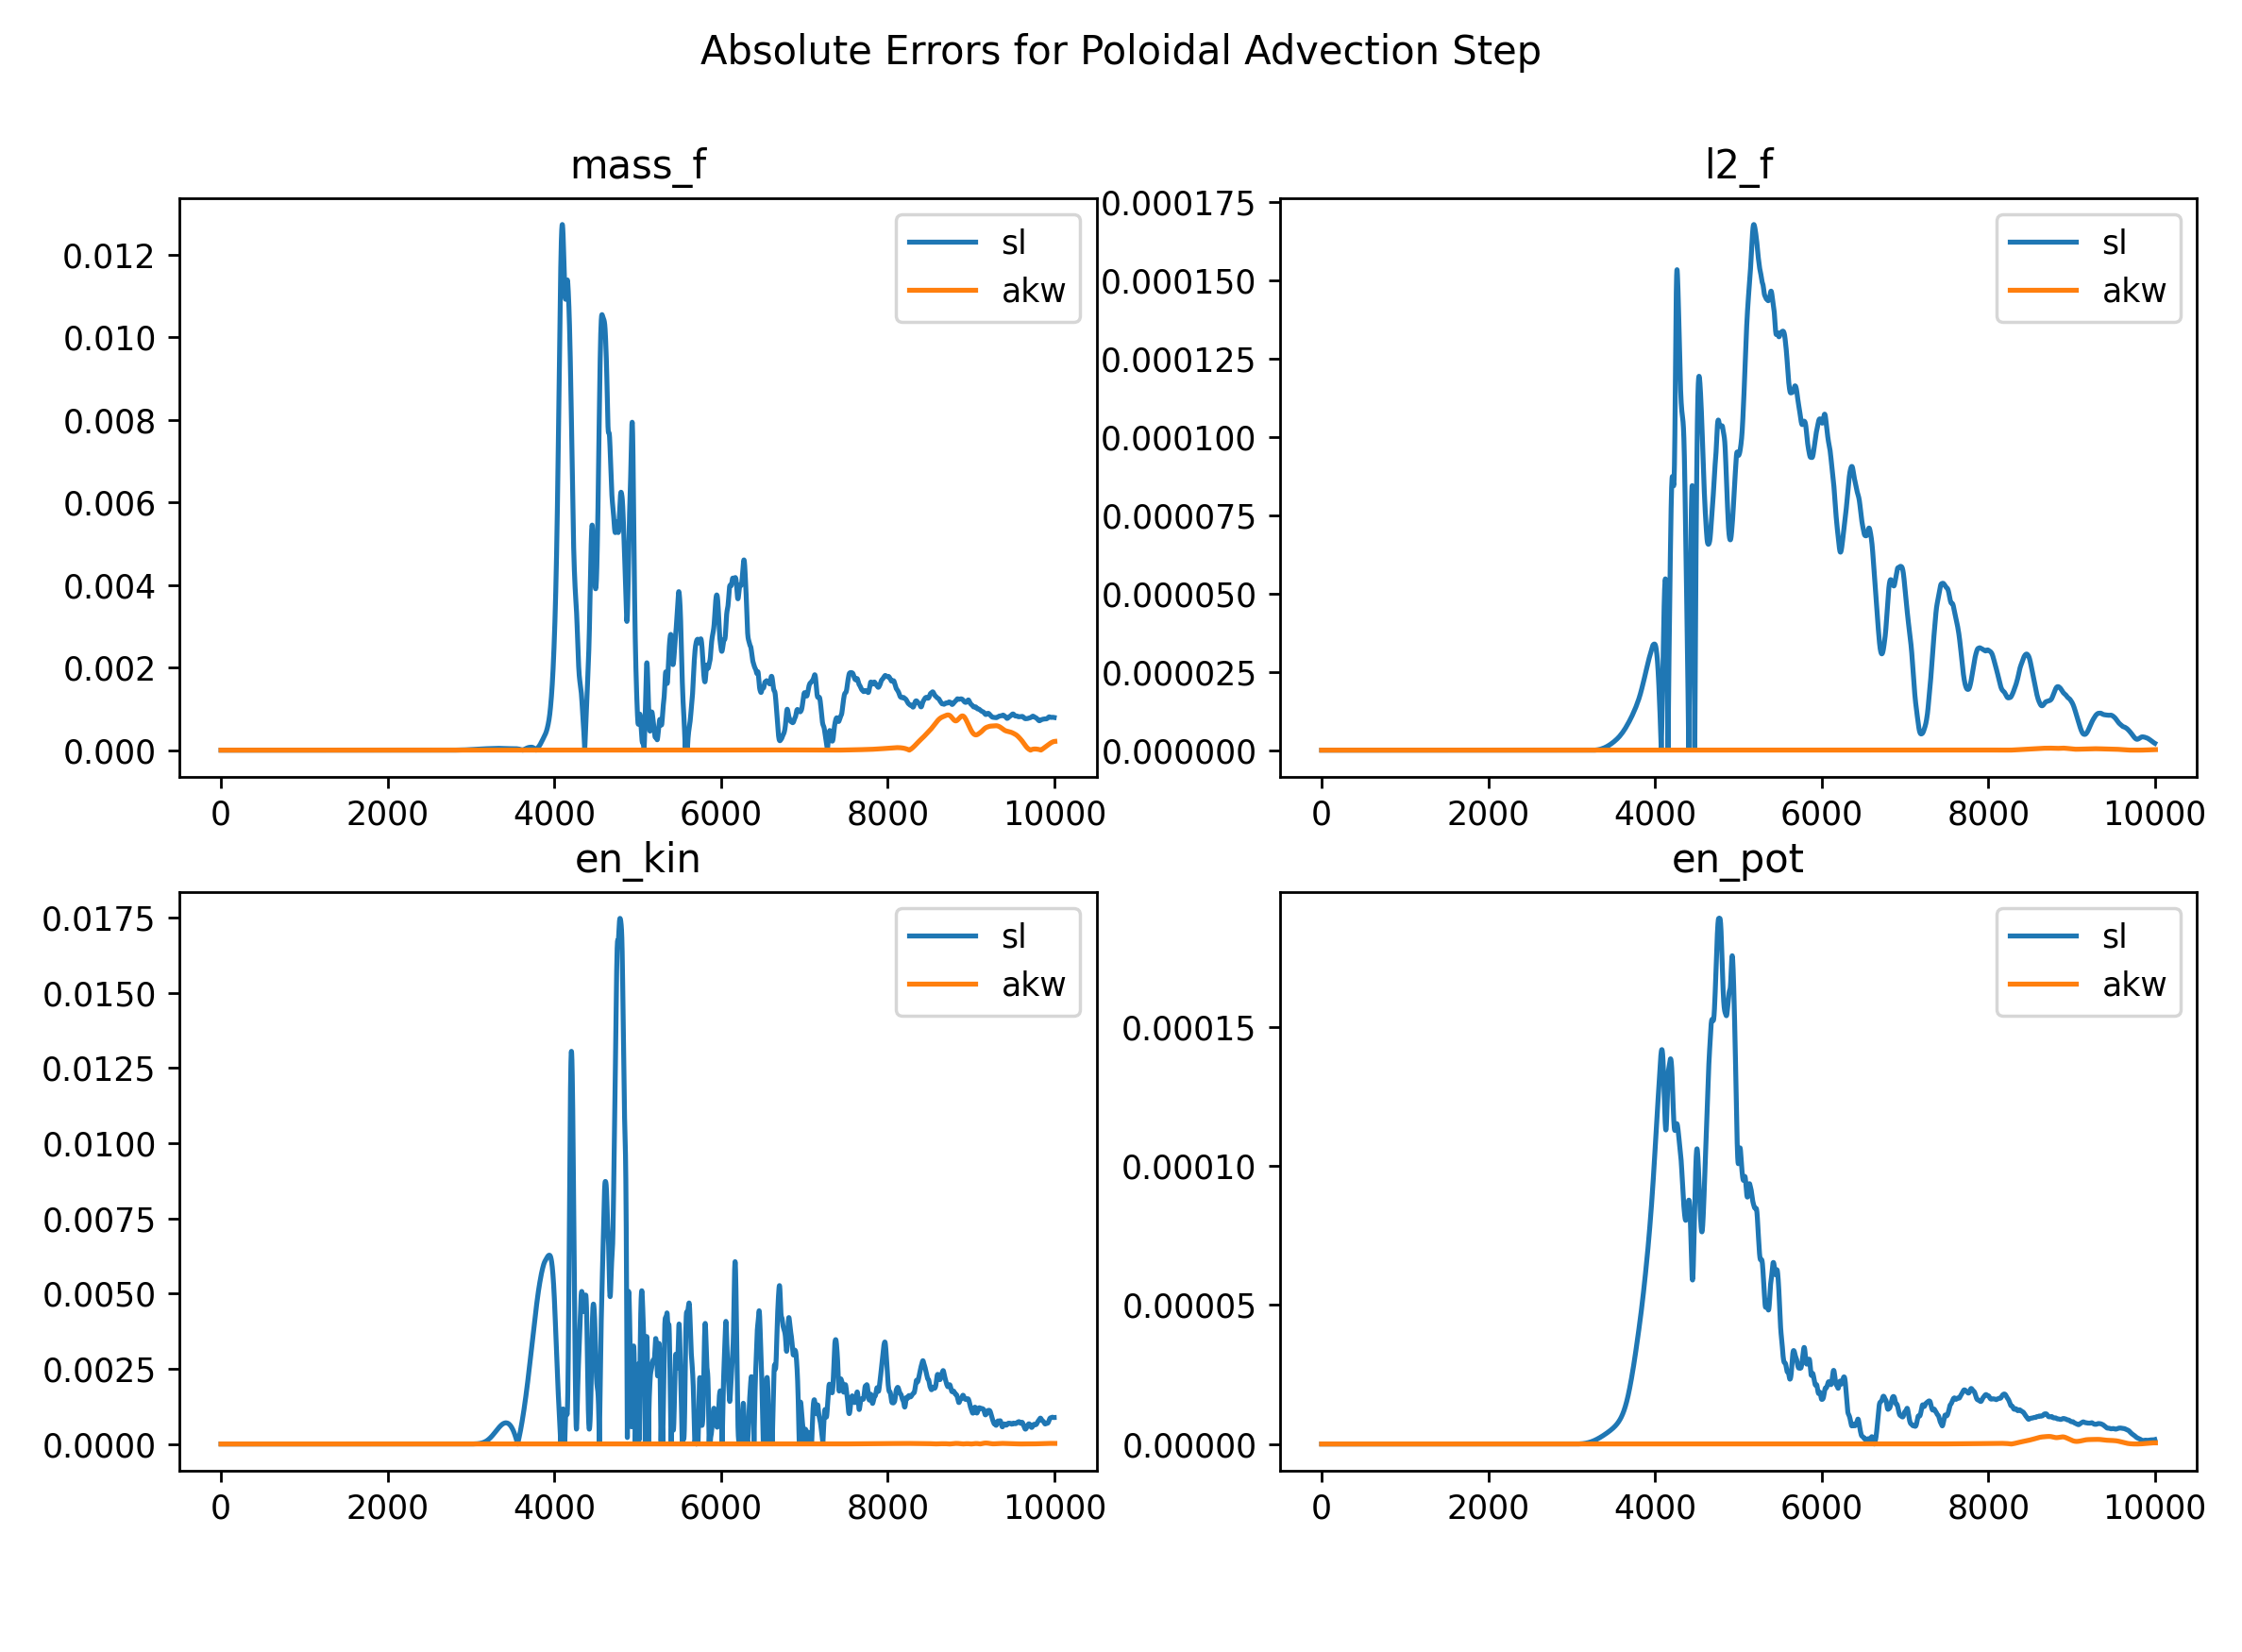
\includegraphics[width=0.9\linewidth]{plots/abs_err}
	\caption{The absolute error for different quantities before and after the poloidal advection step.}
	\label{fig:abserr}
\end{figure}


\begin{figure}
	\centering
	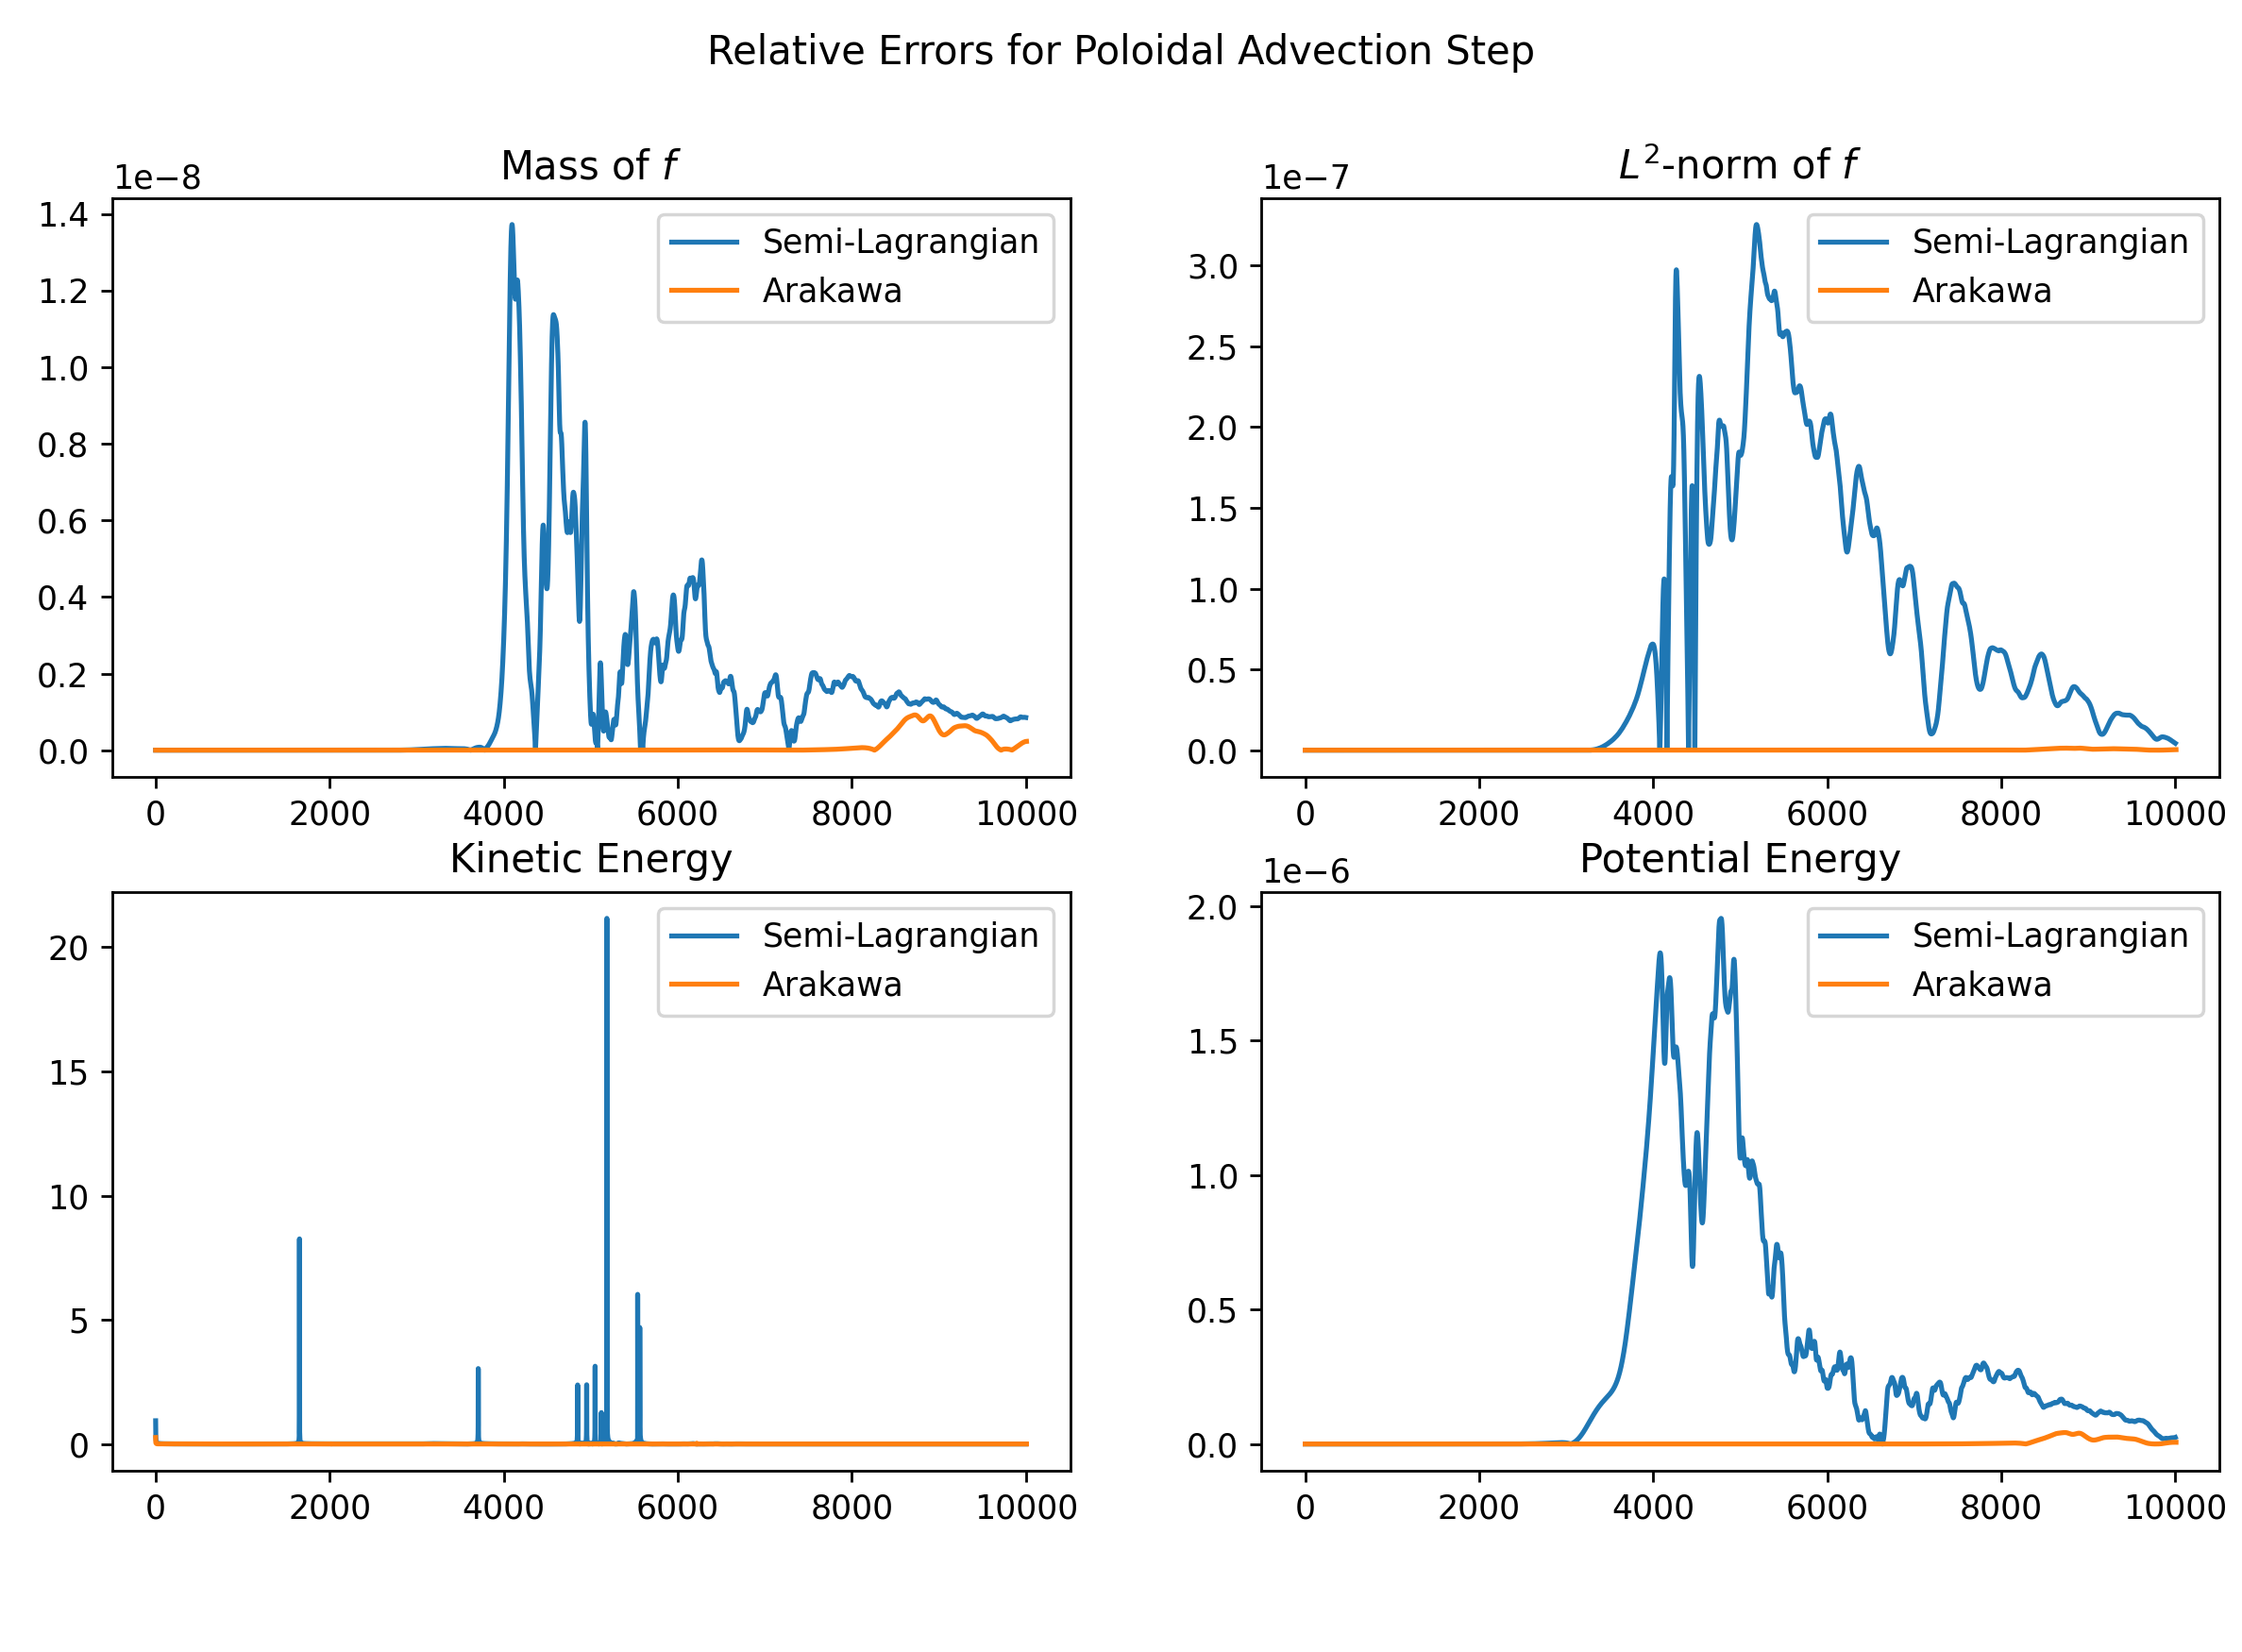
\includegraphics[width=0.9\linewidth]{plots/rel_err}
	\caption{The relative error for different quantities before and after the poloidal advection step.}
	\label{fig:relerr}
\end{figure}


\begin{figure}
	\centering
	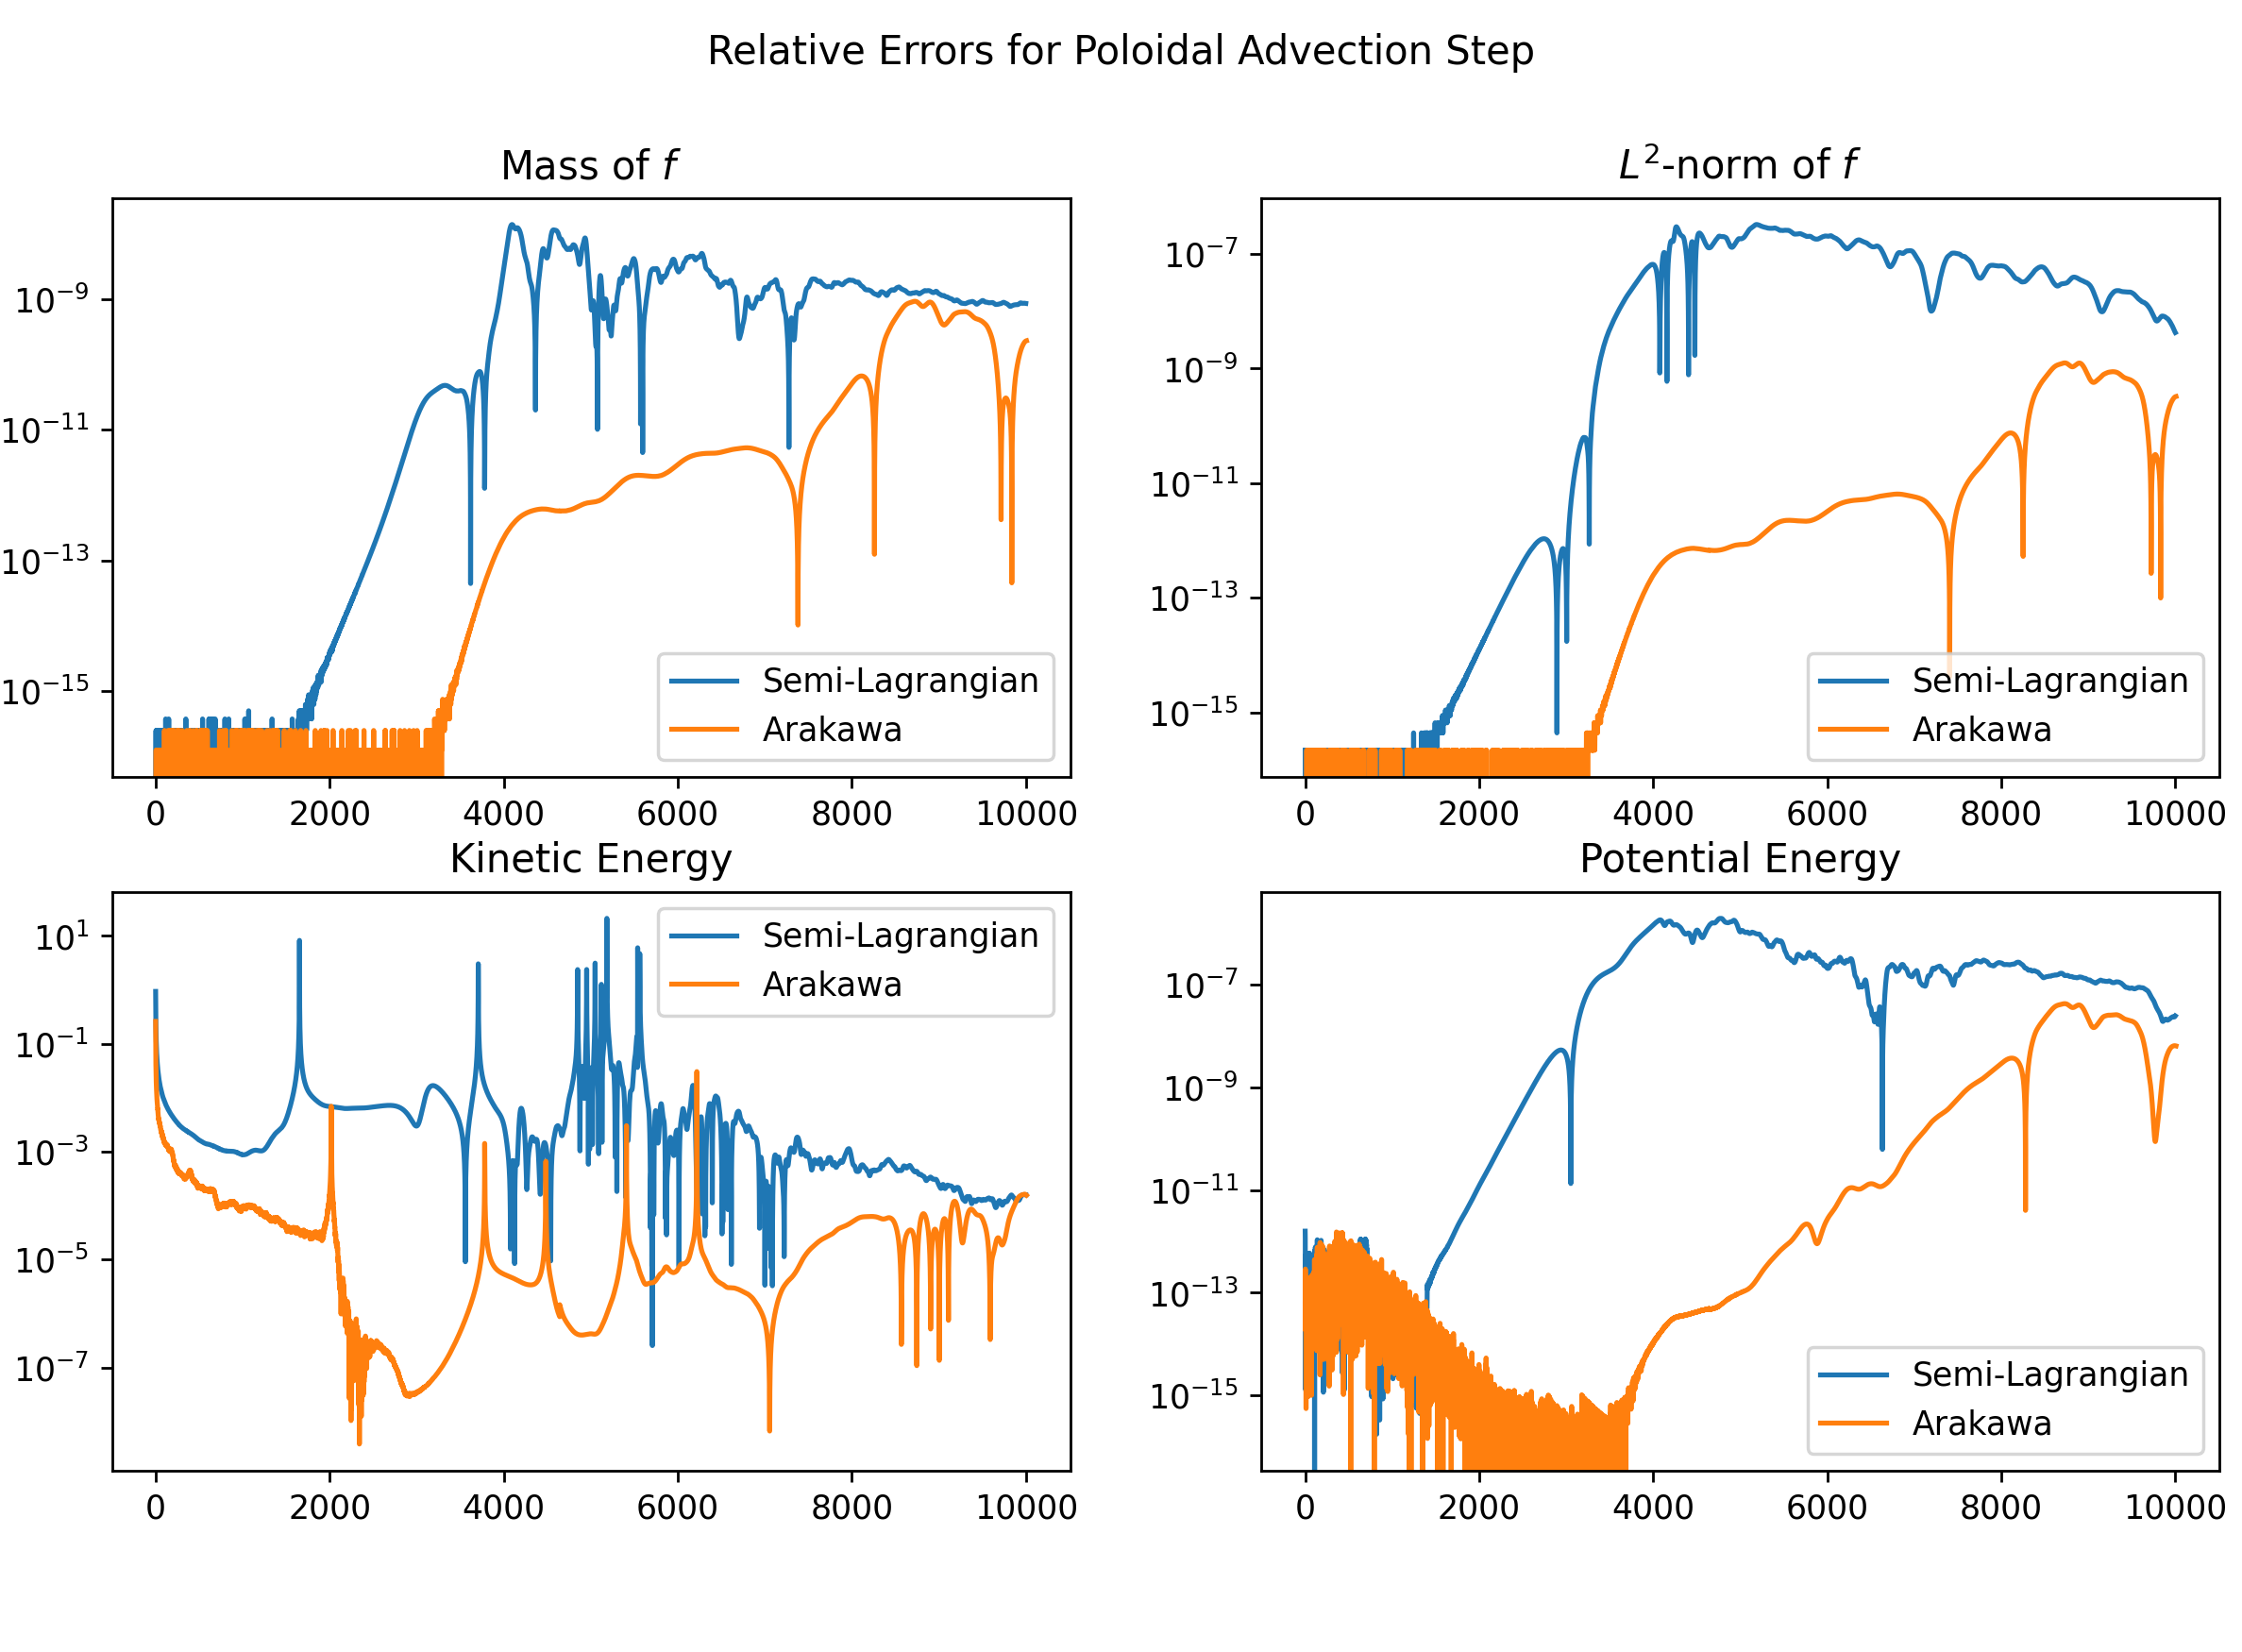
\includegraphics[width=0.9\linewidth]{plots/rel_err_log}
	\caption{The relative error for different quantities before and after the poloidal advection step on a semi-logarithmic scale.}
	\label{fig:relerrlog}
\end{figure}


\begin{figure}
	\centering
	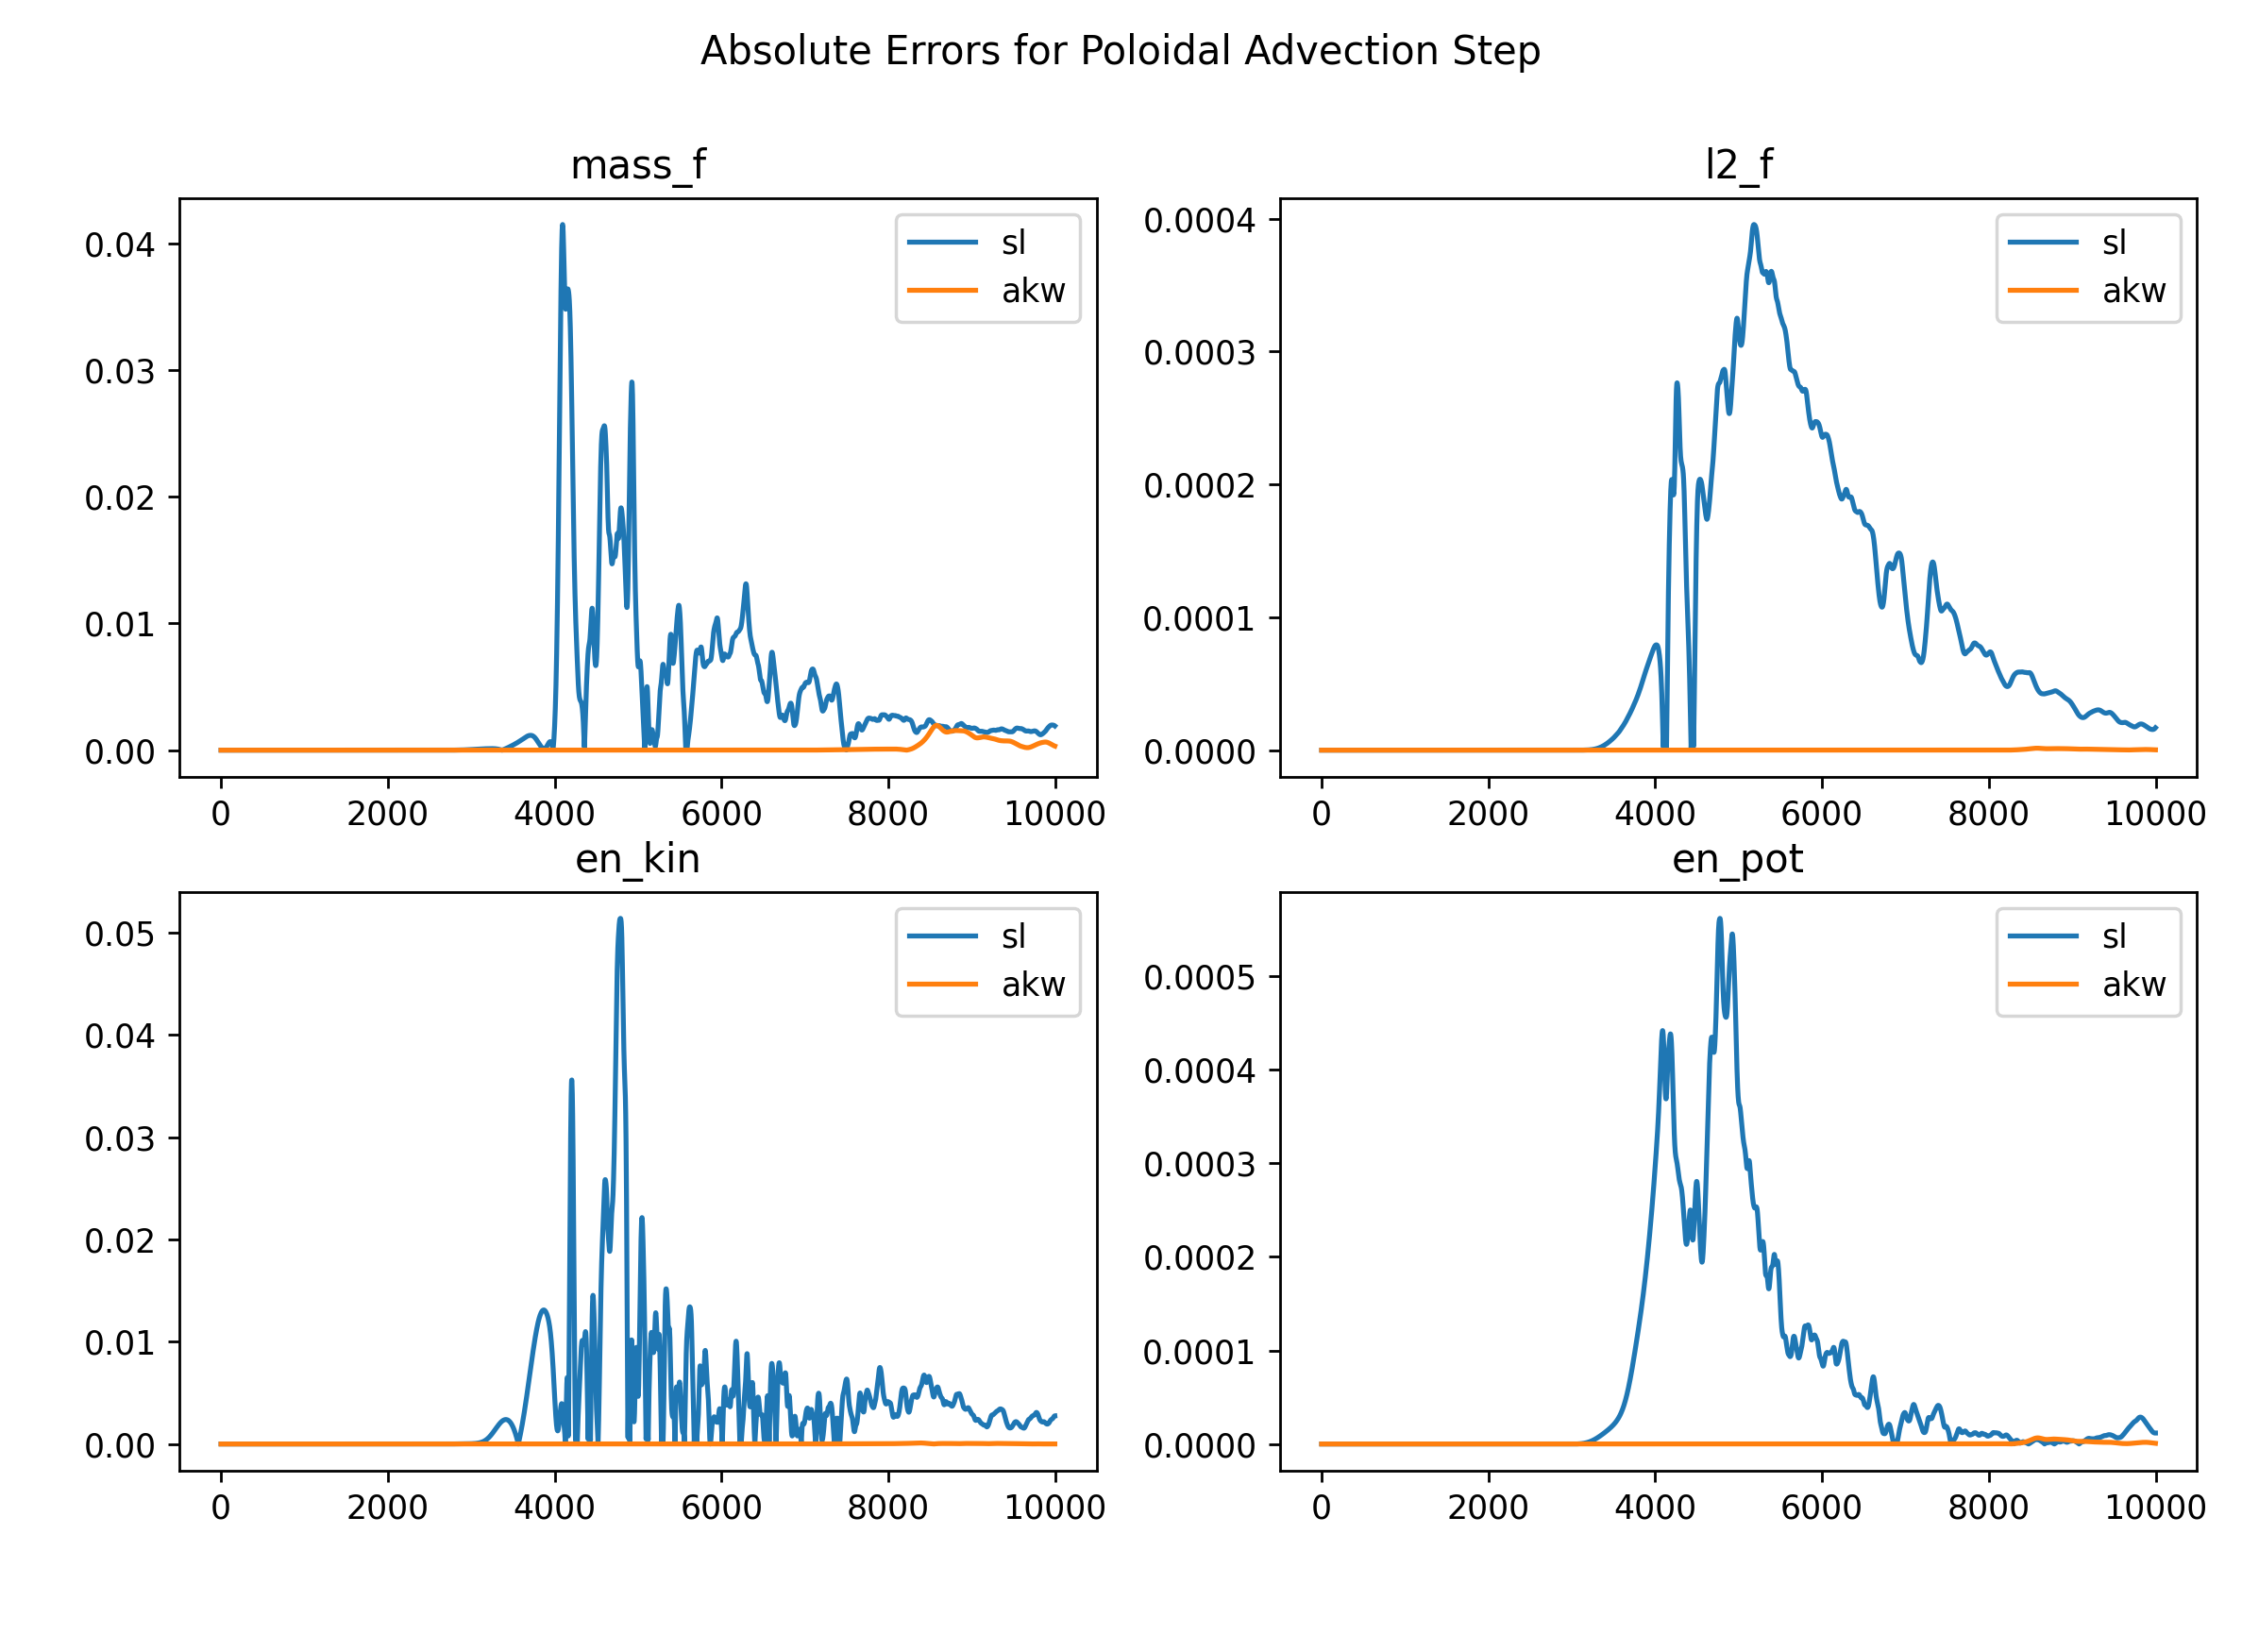
\includegraphics[width=0.9\linewidth]{plots/abs_err dt2}
	\caption{The absolute error for different quantities before and after the poloidal advection step with time step-size $\Delta t = 2$.}
	\label{fig:abserr_dt2}
\end{figure}


\begin{figure}
	\centering
	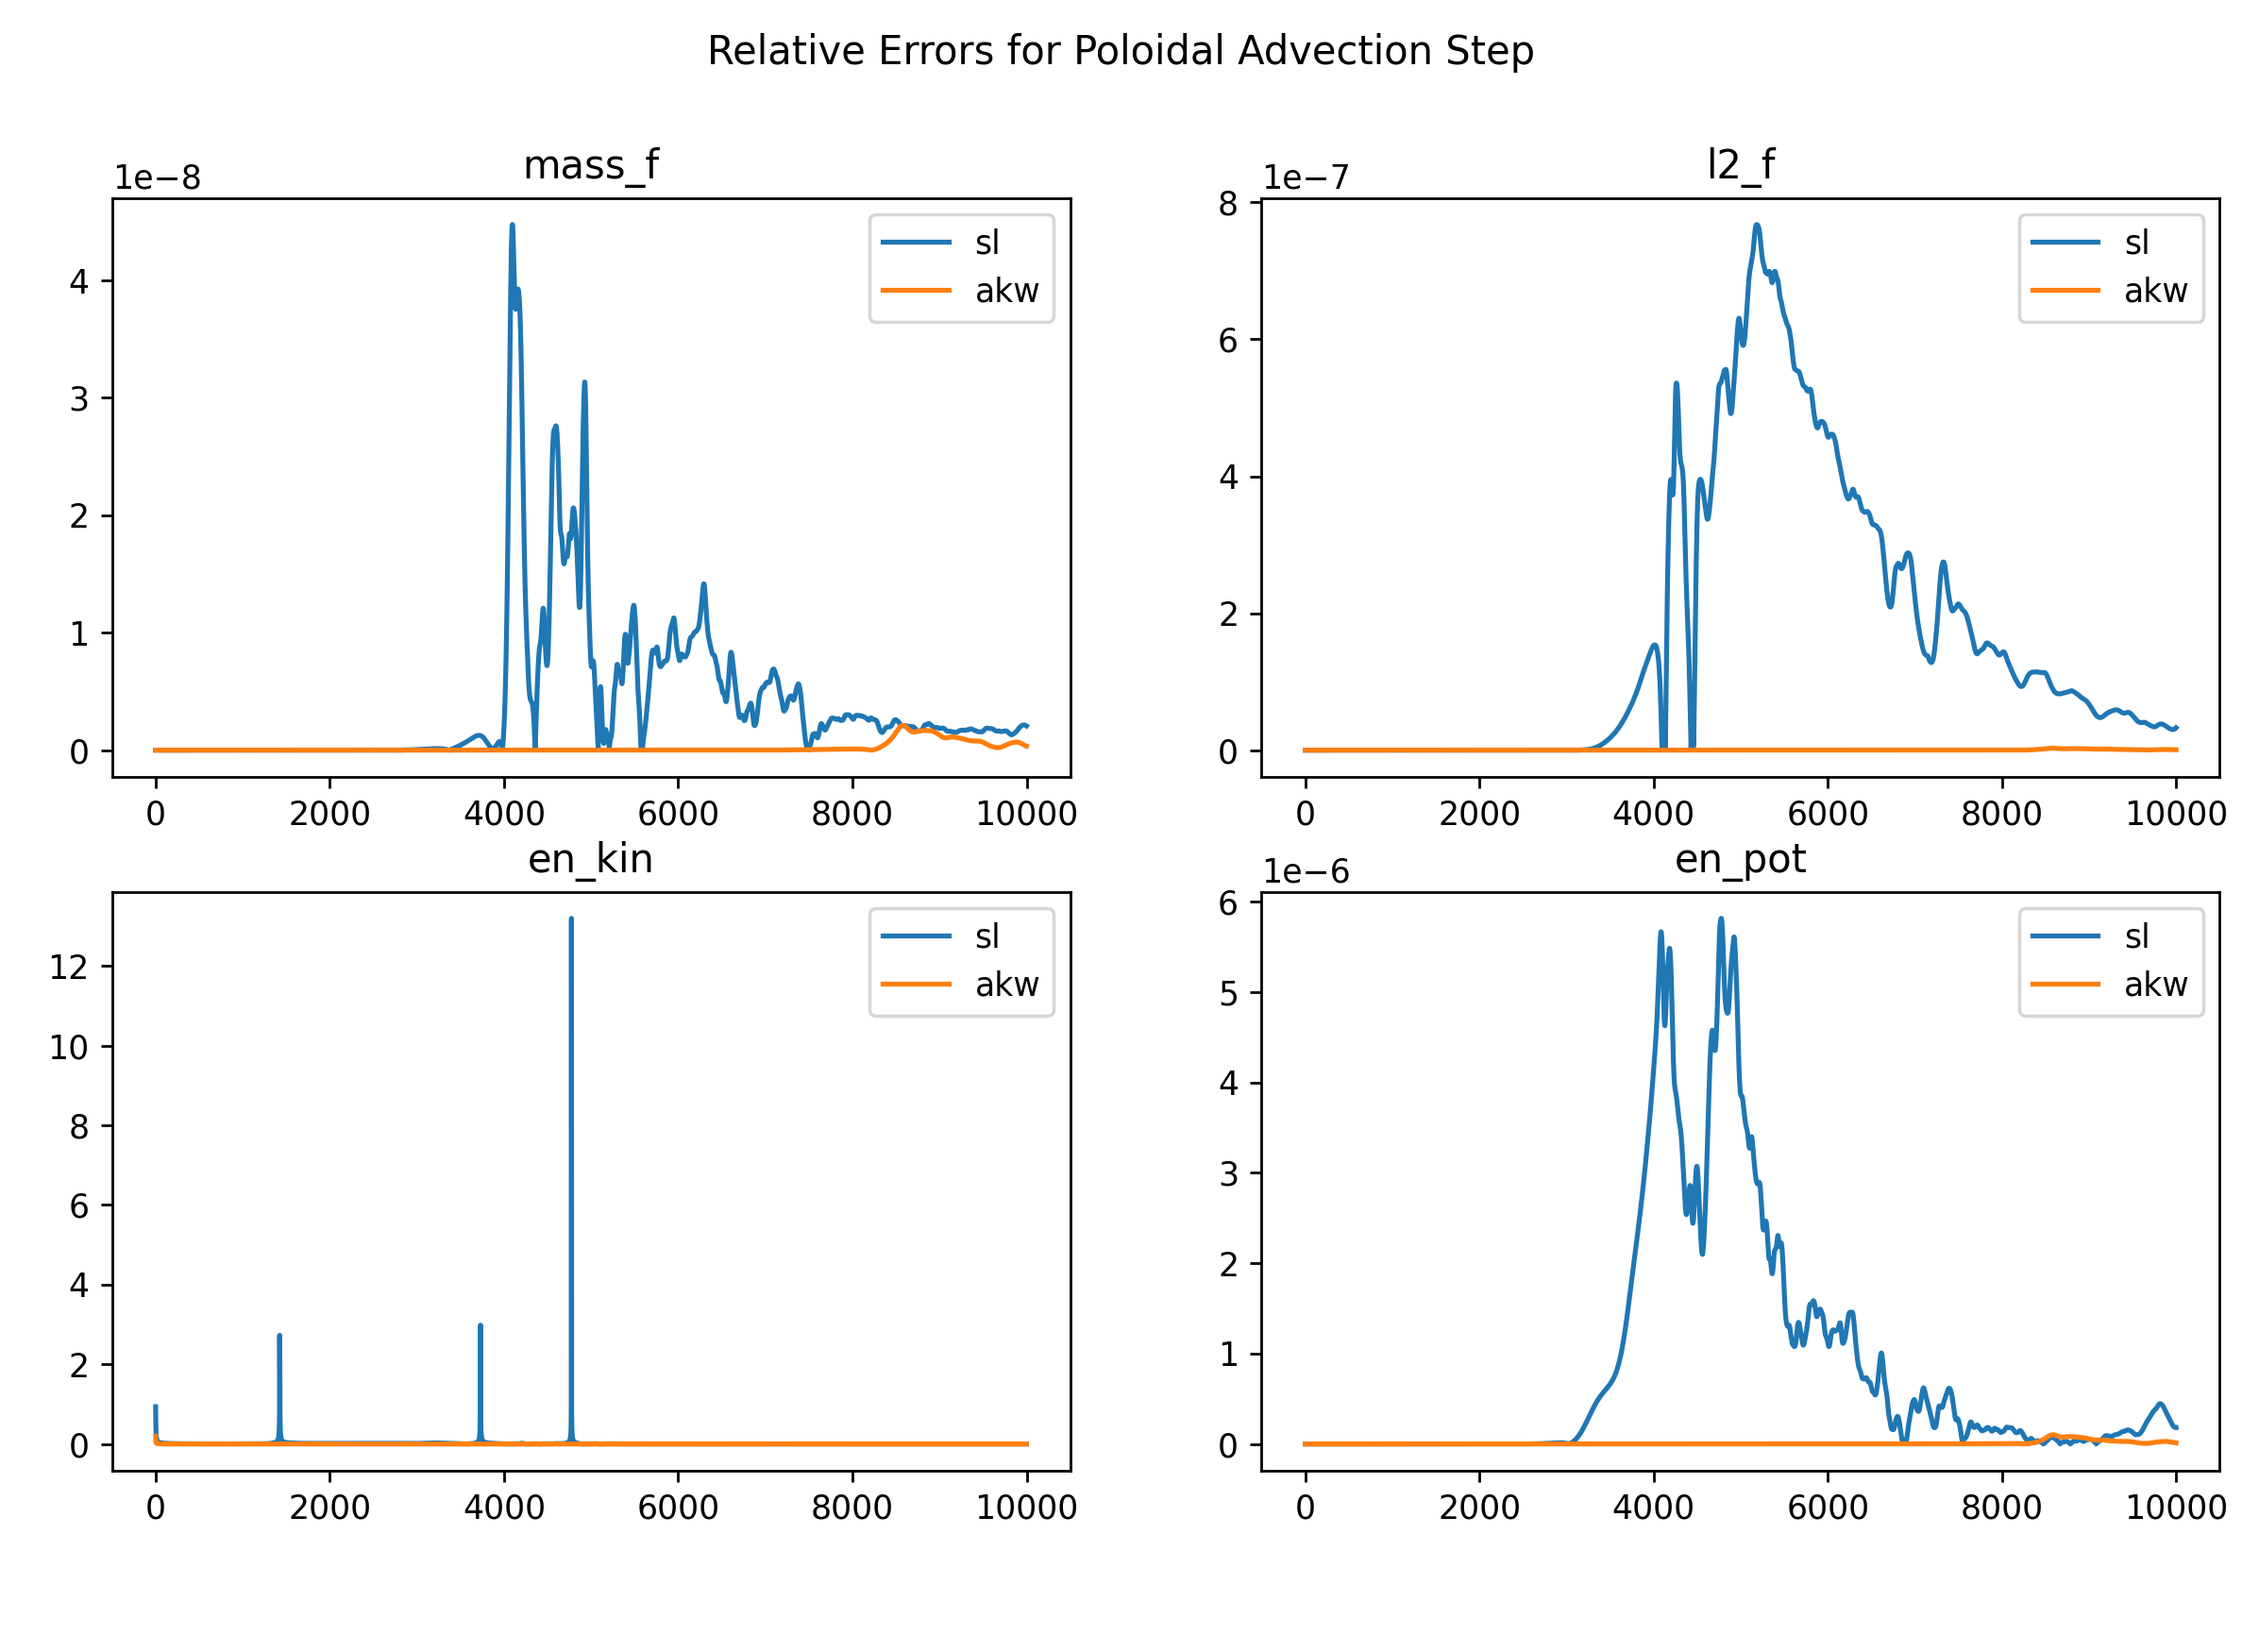
\includegraphics[width=0.9\linewidth]{plots/rel_err dt2}
	\caption{The relative error for different quantities before and after the poloidal advection step with time step-size $\Delta t = 2$.}
	\label{fig:relerr_dt2}
\end{figure}


\begin{figure}
	\centering
	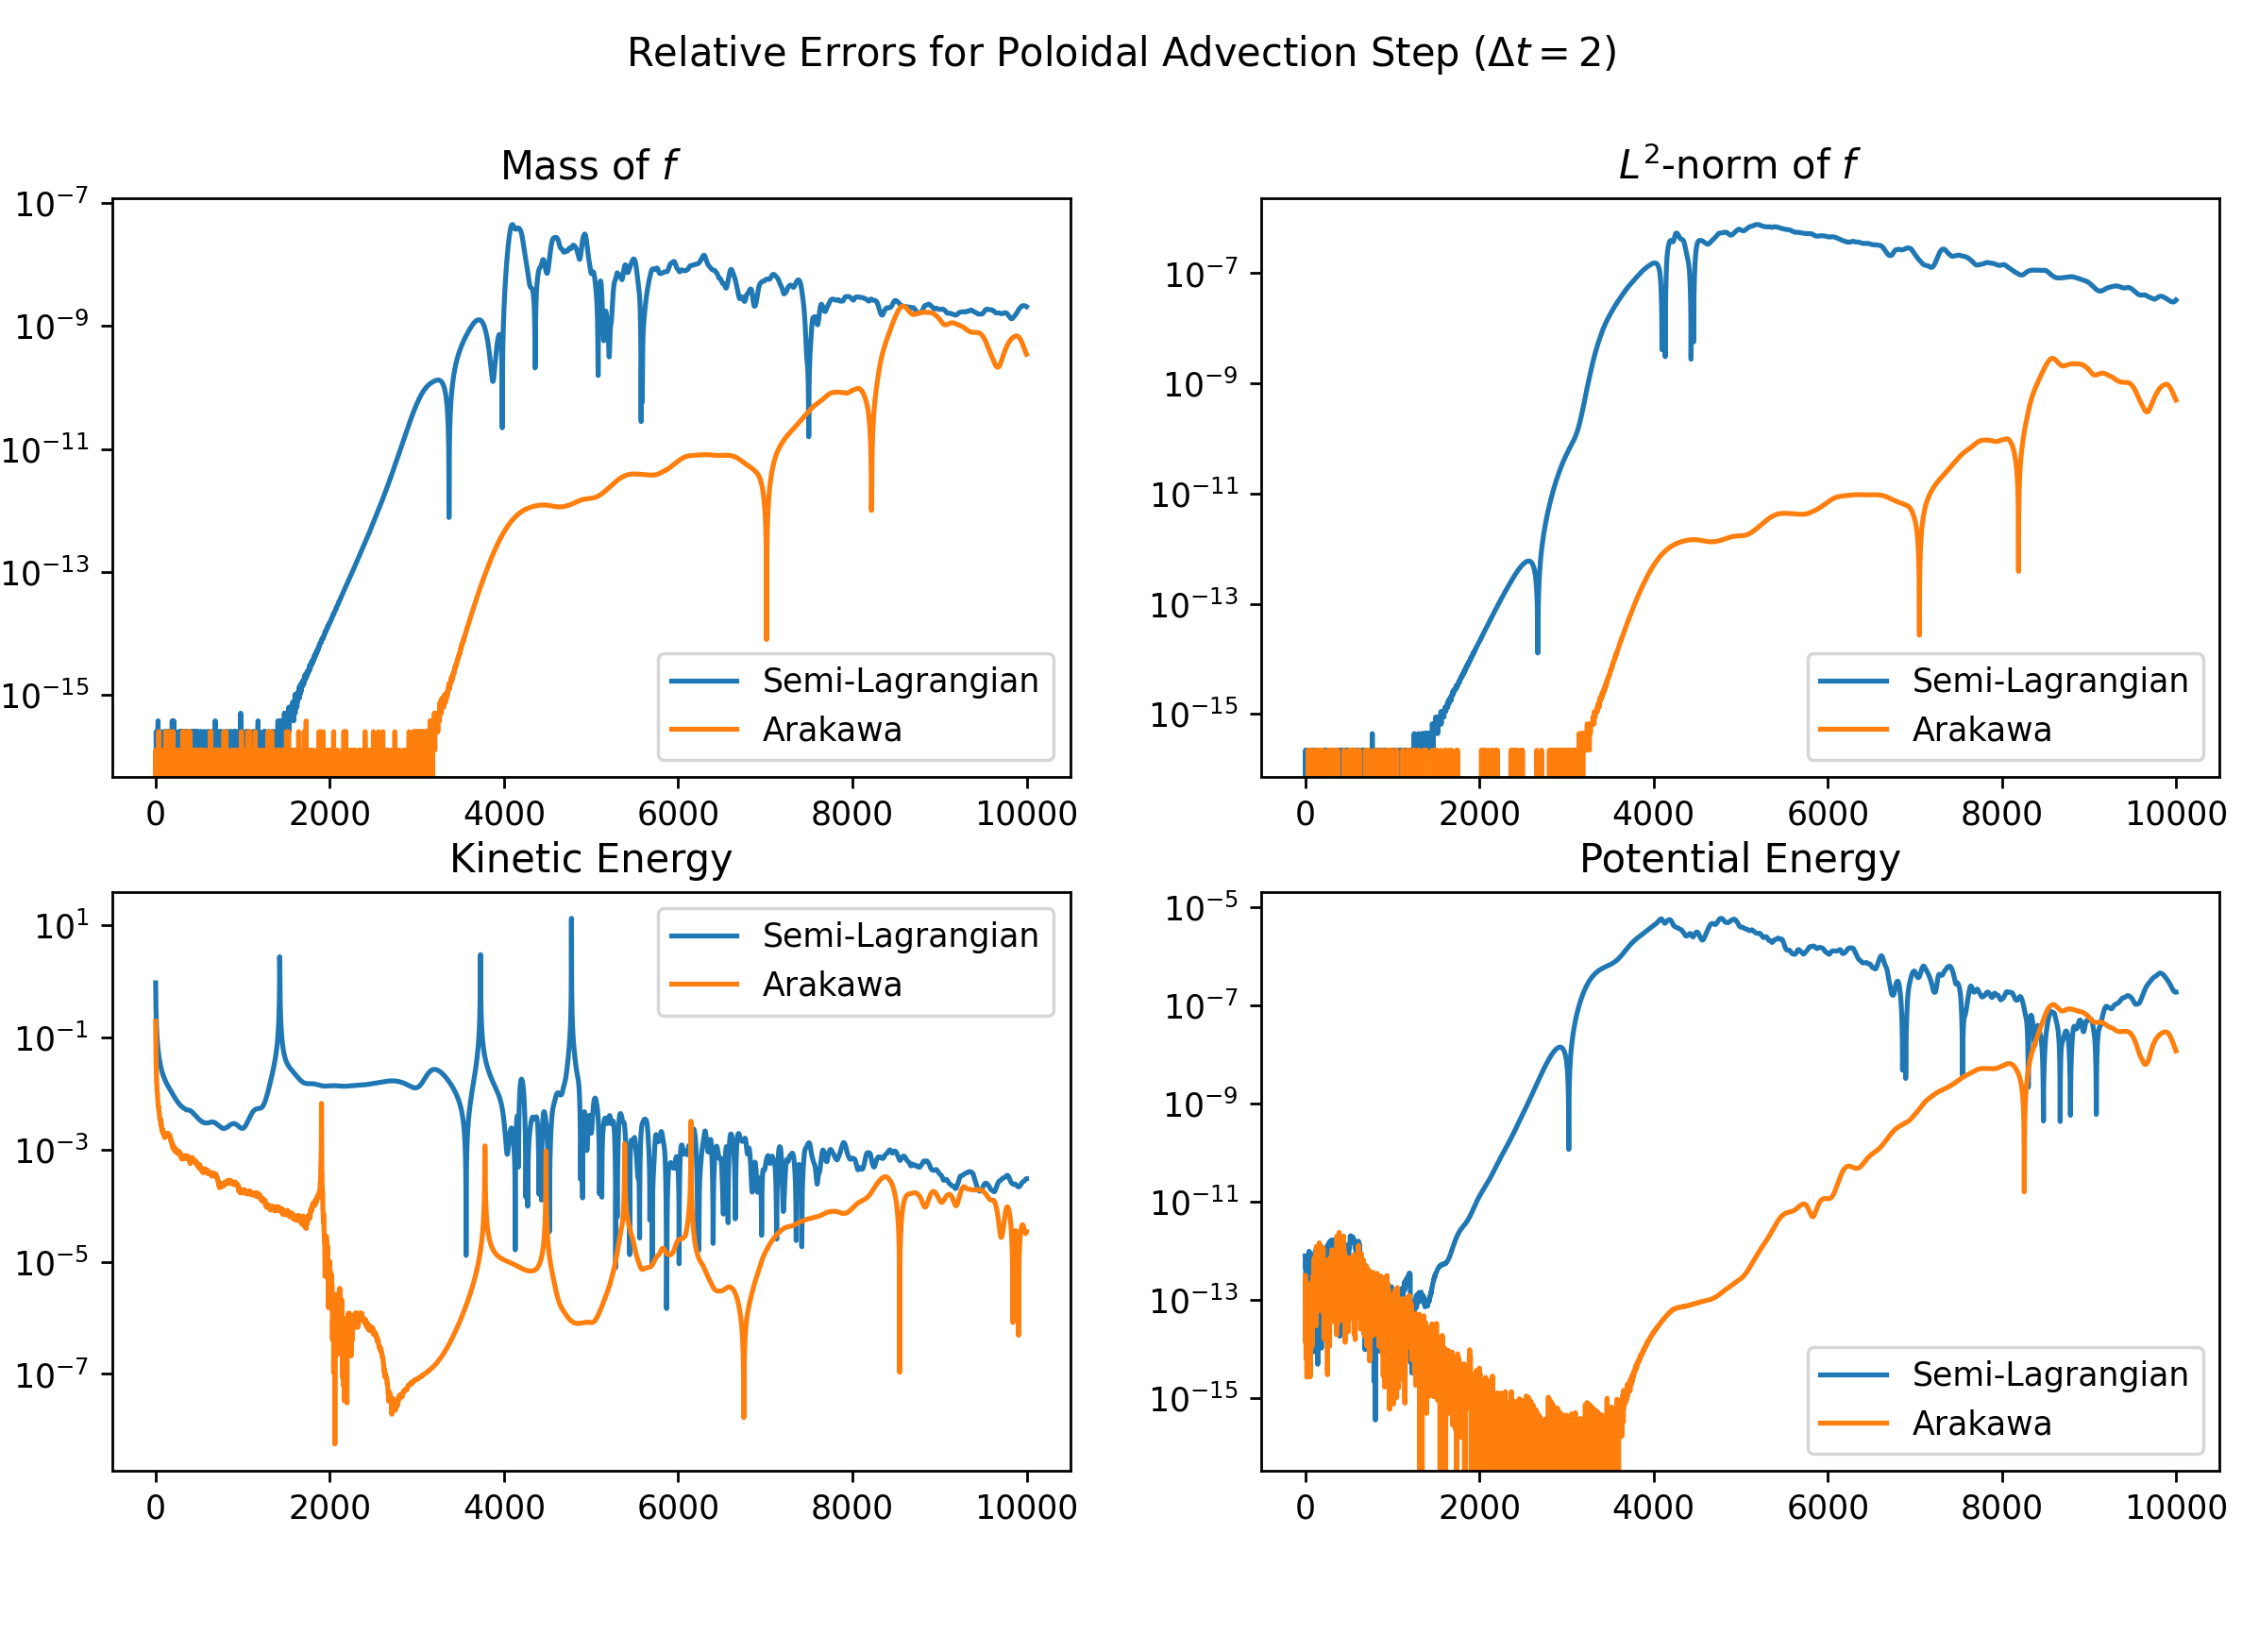
\includegraphics[width=0.9\linewidth]{plots/rel_err_log dt2}
	\caption{The relative error for different quantities before and after the poloidal advection step on a semi-logarithmic scale with time step-size $\Delta t = 2$.}
	\label{fig:relerrlog_dt2}
\end{figure}


\begin{figure}
	\centering
	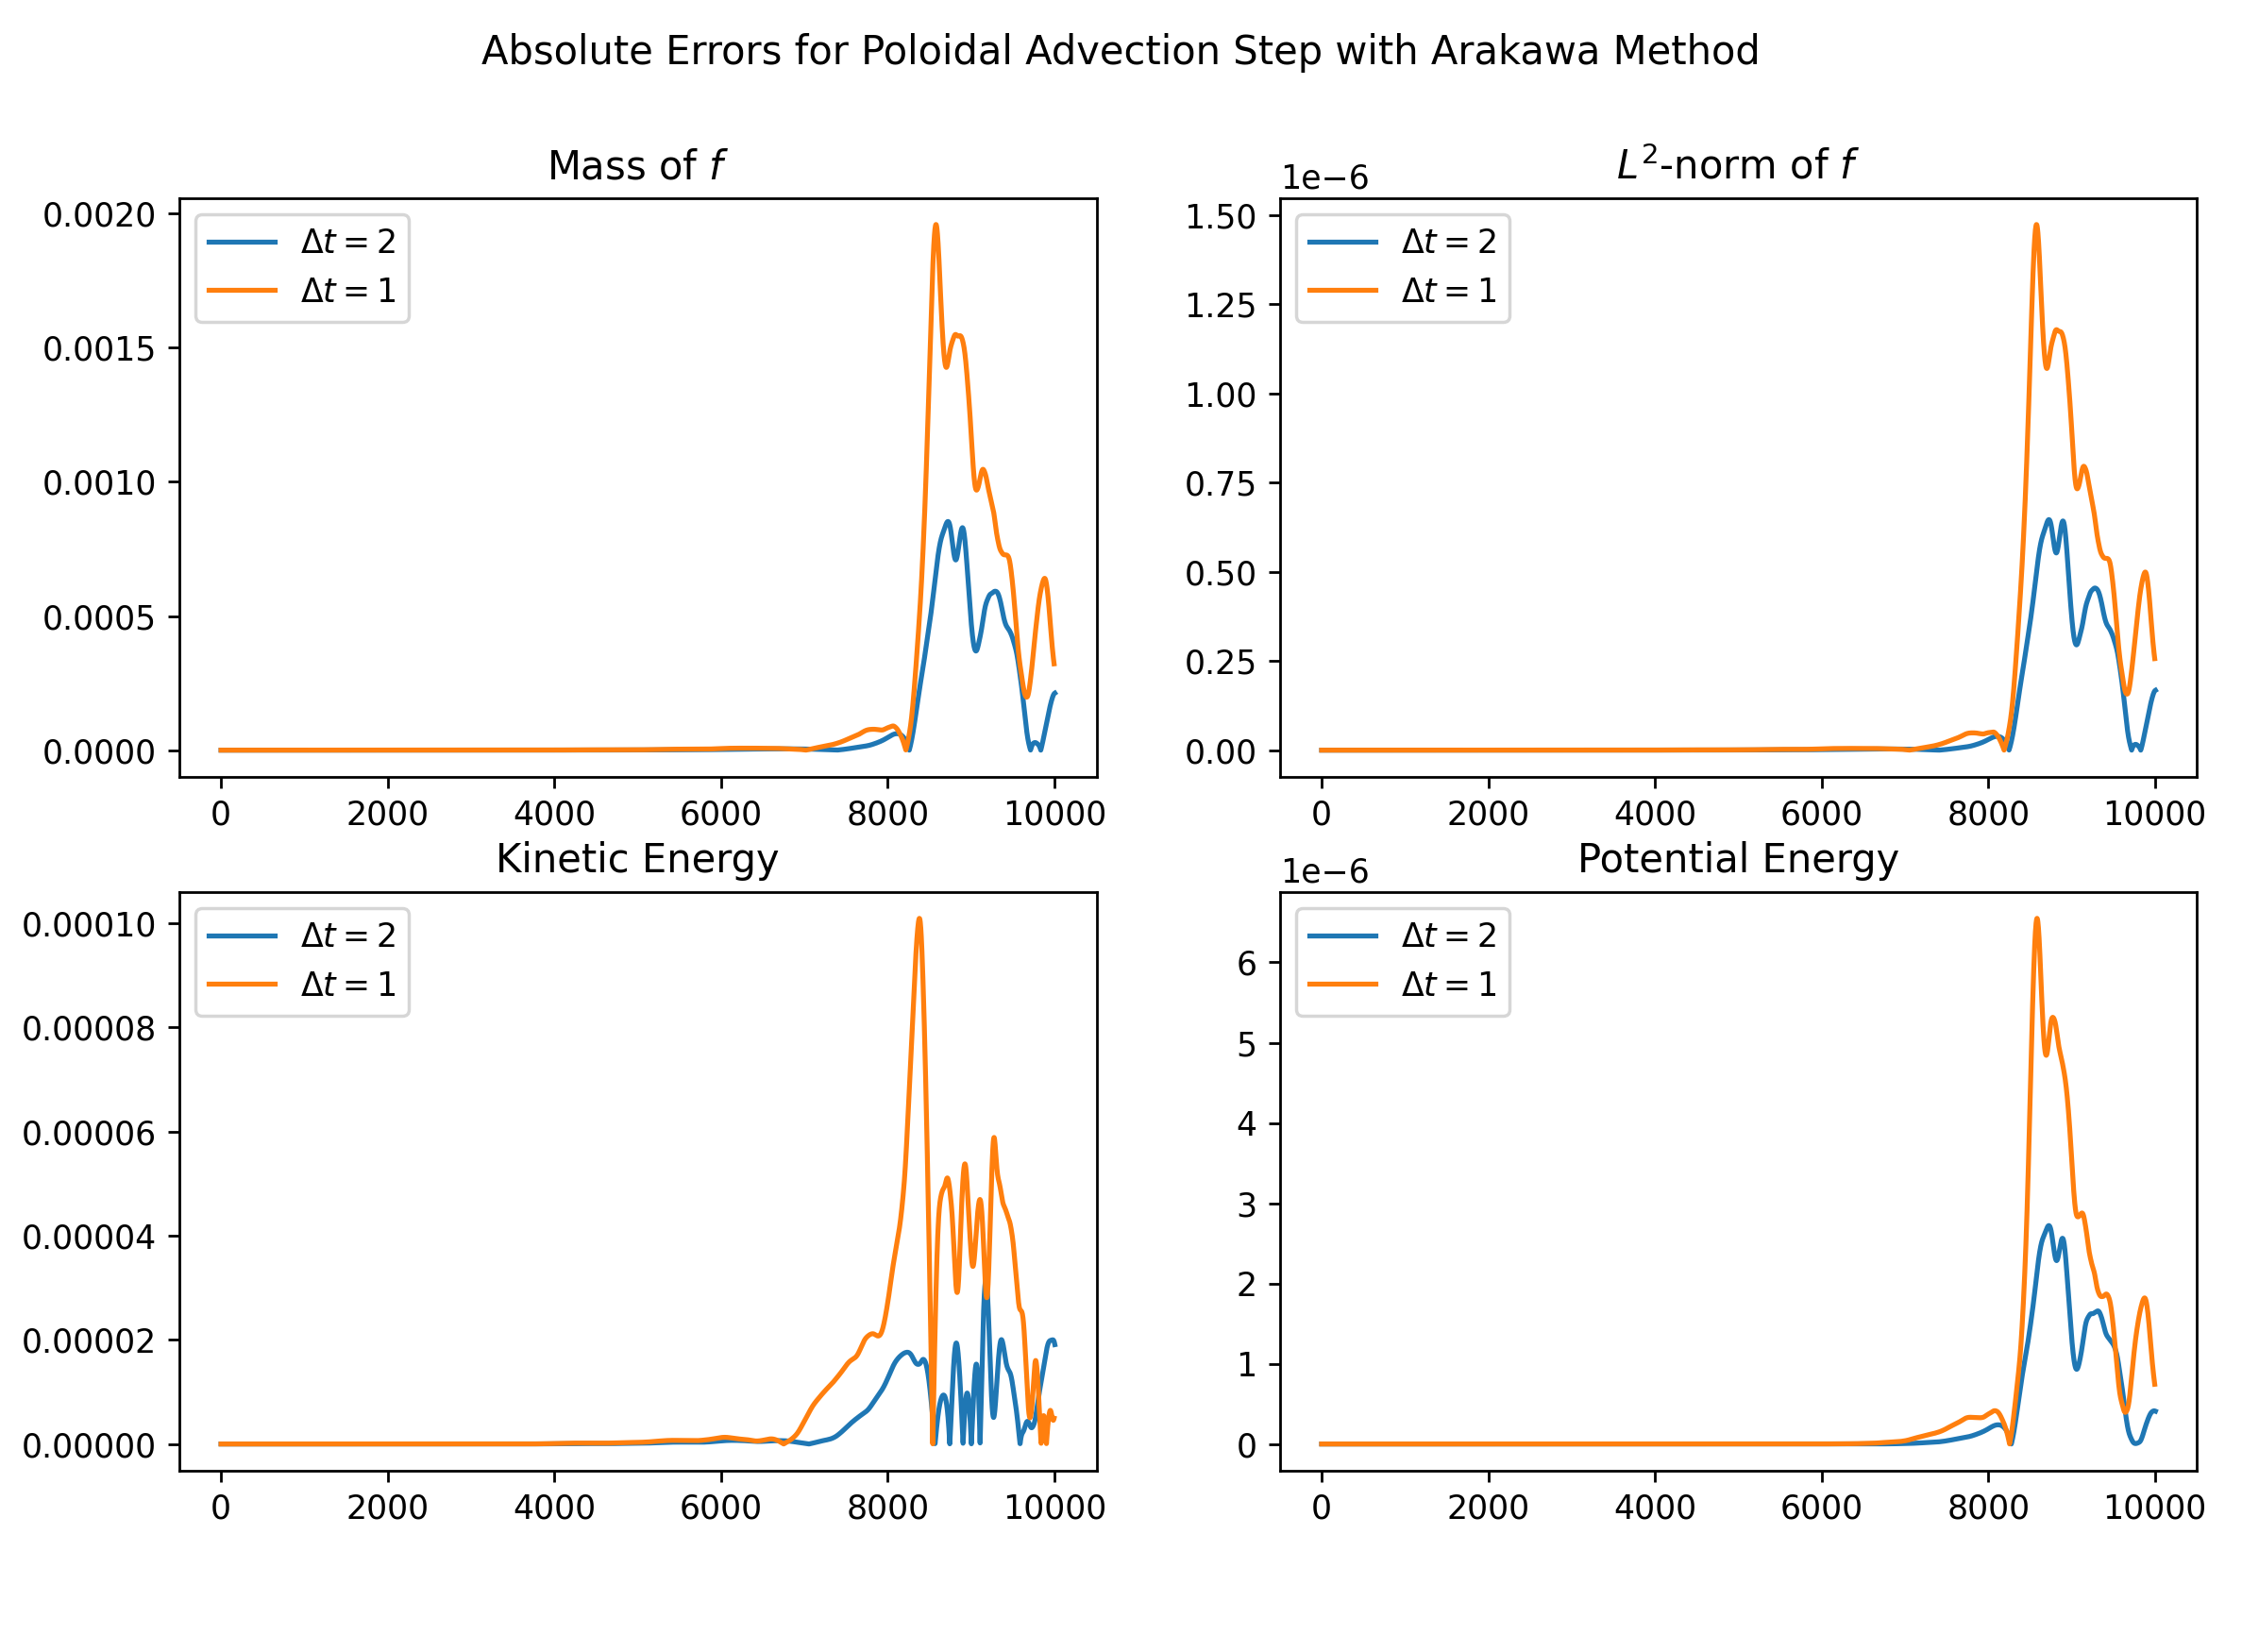
\includegraphics[width=0.9\linewidth]{plots/abs_err akw}
	\caption{The absolute error for different quantities before and after the poloidal advection step with the Arakawa method, comparing time step-size $\Delta t = 1$ and $\Delta t = 2$.}
	\label{fig:abserr_akw}
\end{figure}


\begin{figure}
	\centering
	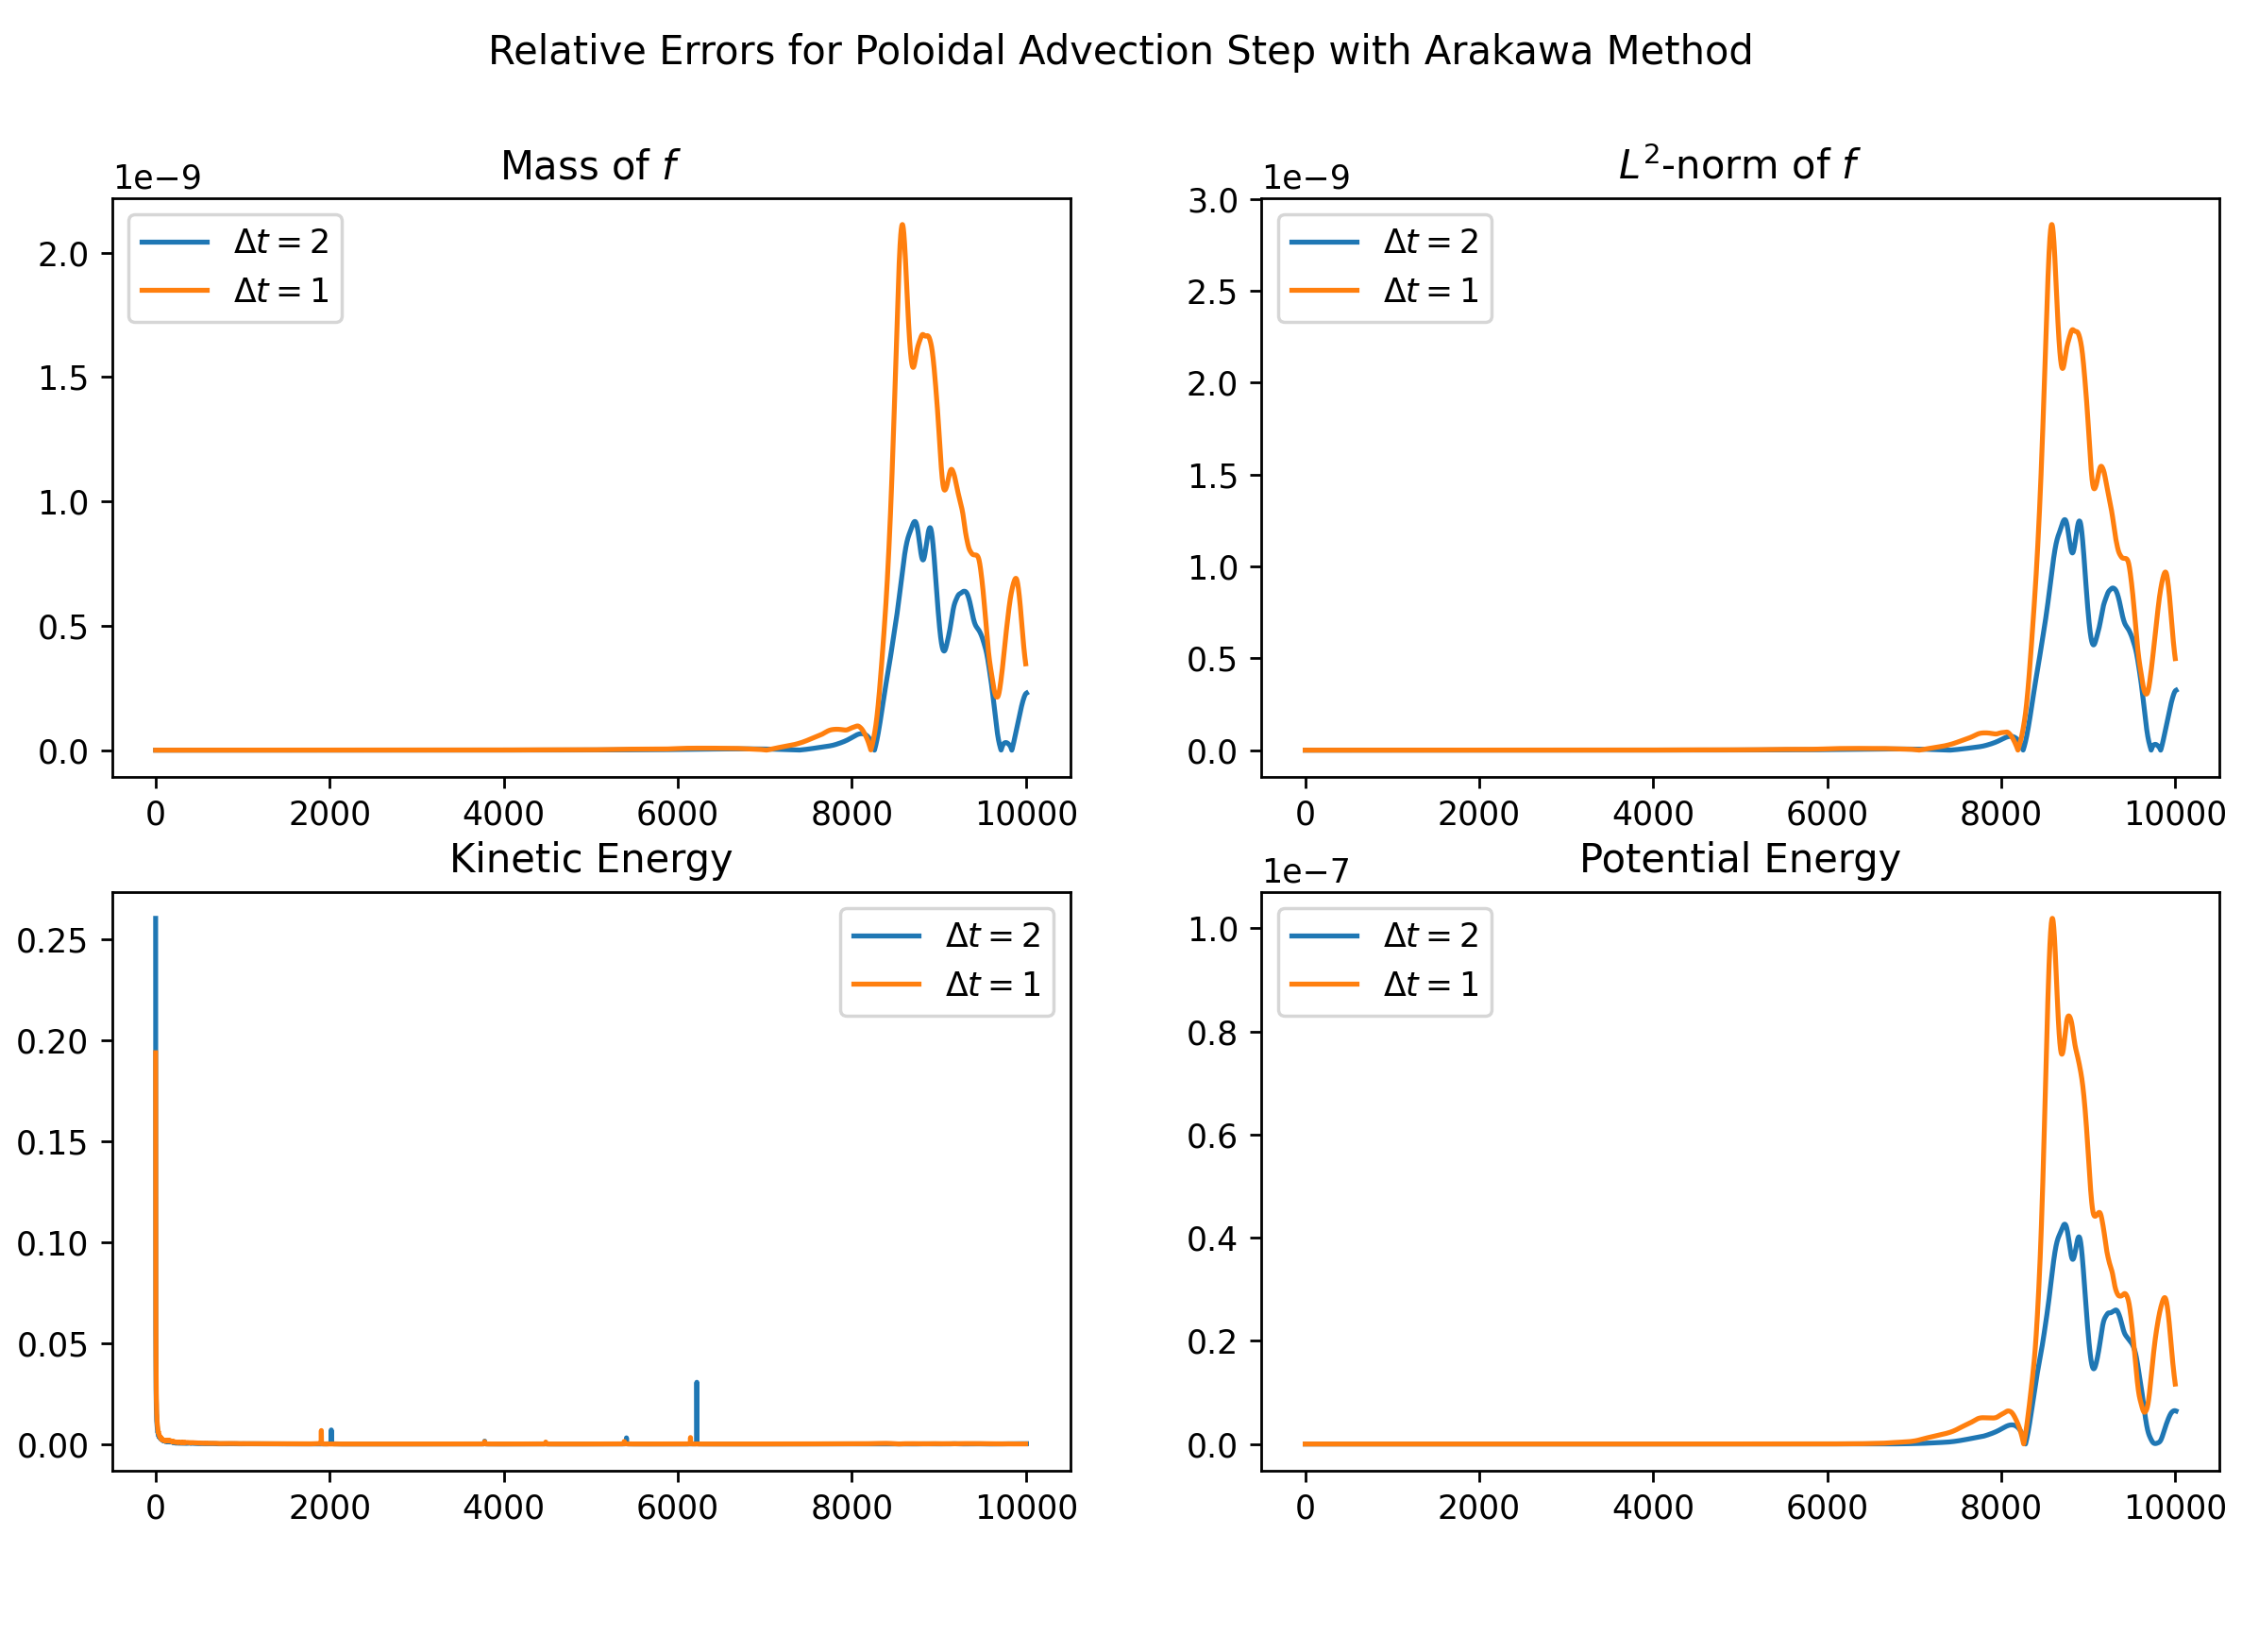
\includegraphics[width=0.9\linewidth]{plots/rel_err akw}
	\caption{The relative error for different quantities before and after the poloidal advection step with the Arakawa method, comparing time step-size $\Delta t = 1$ and $\Delta t = 2$..}
	\label{fig:relerr_akw}
\end{figure}


\begin{figure}
	\centering
	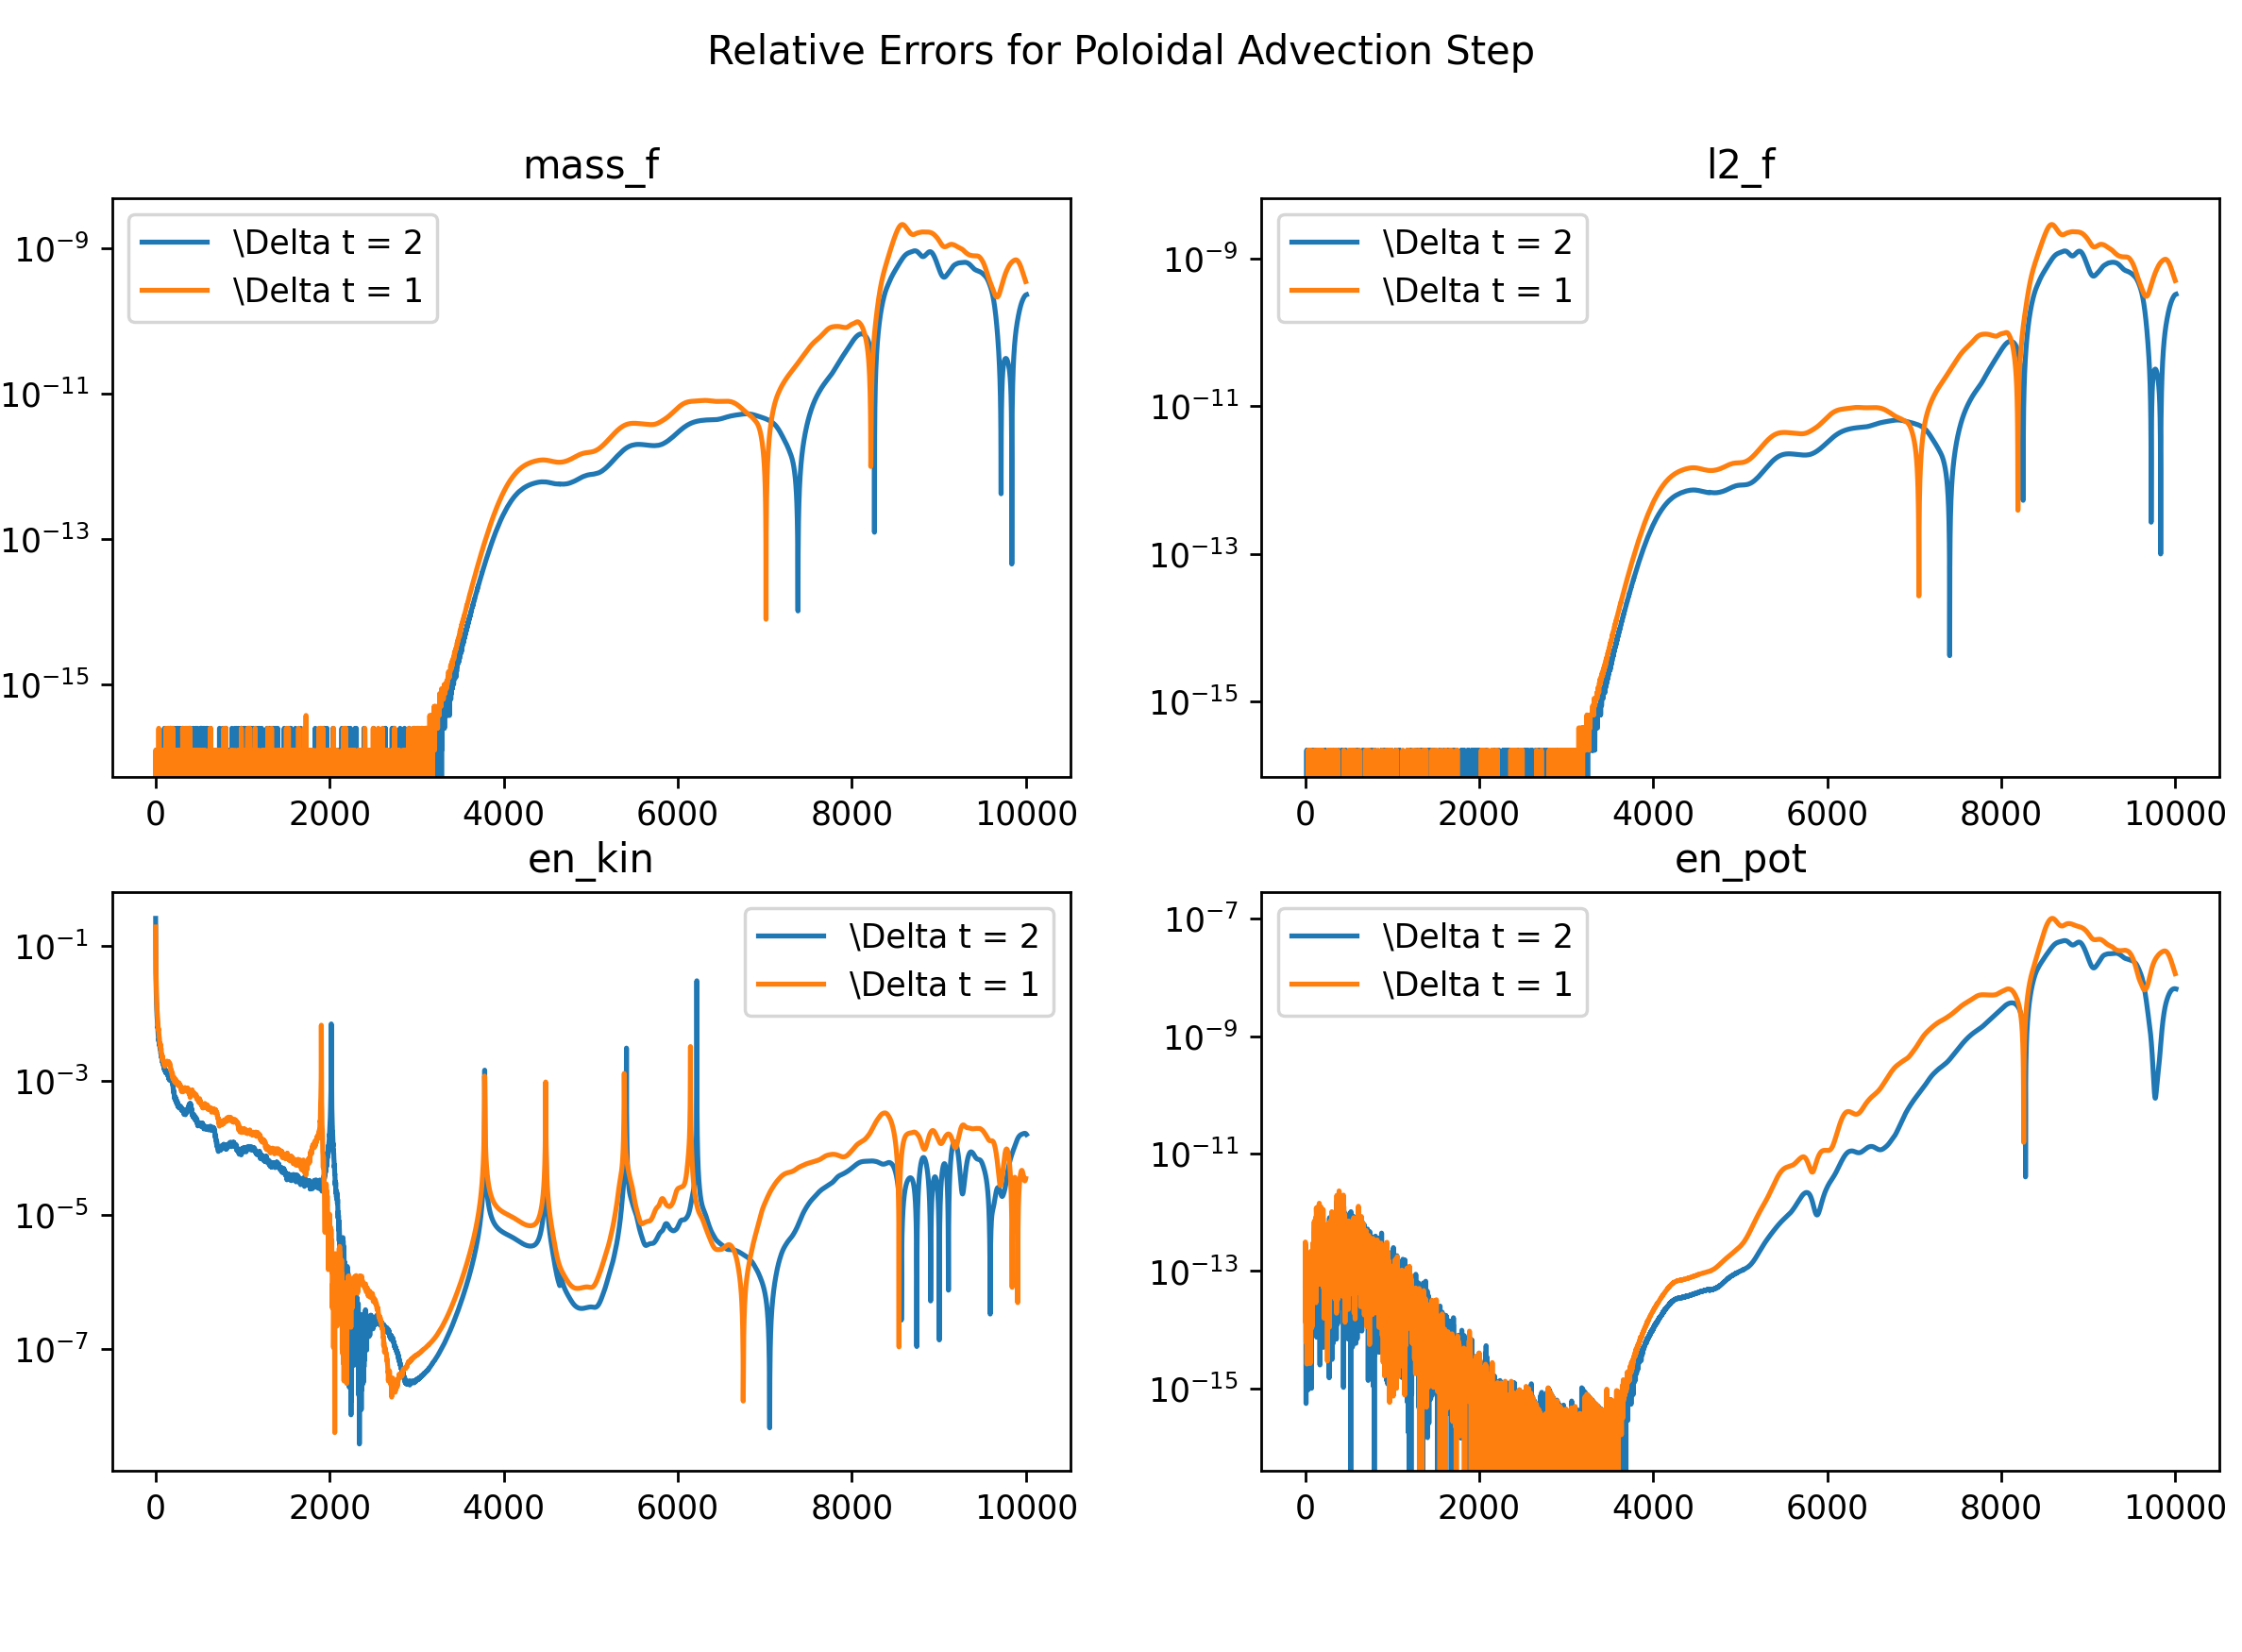
\includegraphics[width=0.9\linewidth]{plots/rel_err_log akw}
	\caption{The relative error for different quantities before and after the poloidal advection step on a semi-logarithmic scale with the Arakawa method, comparing time step-size $\Delta t = 1$ and $\Delta t = 2$..}
	\label{fig:relerrlog_akw}
\end{figure}





\section{Conclusion}
\label{sec:conclusion}

Bonne travaille, je suis très satisfée.


\begin{acknowledgement}
	\textbf{Acknowledgements}\\
	The authors would like to thank Emmanuel Franck, Hélène Hivert, Guillaume Latu, Hélène Leman, Bertrand Maury, Michel Mehrenberger, and Laurent Navoret for organizing the CEMRACS conference 2022 and for the wonderful opportunity to come to Marseille and do research. We express special thanks to Michel Mehrenberger, Virginie Grandgirard, and Martin Campos Pinto for the daily supervision and general shaping of the project. Dominik Bell and Frederik Schnack thank Eric Sonnendrücker for the opportunity to participate in the CEMRACS and the fruitful discussions after the conference to give this project the final details. All authors are tremendously thankful for Emily Bourne and her help with the implementation and the work she did on the PyGyro code, which laid the ground-work for this project.
\end{acknowledgement}

\bibliographystyle{ieeetr}
\bibliography{literature}
\end{document}
